\documentclass{amsart}
\usepackage[T1]{fontenc}
\usepackage[p,osf]{Baskervaldx}
\usepackage[scale=.875,type1]{cabin}
\usepackage[baskervaldx,vvarbb]{newtxmath}
\usepackage[scr=boondoxo]{mathalfa}
\usepackage{amsmath,amsthm,amsaddr,booktabs}
%\usepackage{amssymb,amsfonts,mathrsfs,stmaryrd}
\usepackage{tikz,tikz-cd}
\usepackage{graphicx}
\usepackage{booktabs}
\newtheorem{lem}{Lemma}
\newtheorem{prop}{Proposition}
\newtheorem{thm}{Theorem}
\newtheorem*{lem*}{Lemma}
\newtheorem*{prop*}{Proposition}
\newtheorem*{thm*}{Theorem}
\theoremstyle{definition}
\newtheorem{defn}{Definition}
\def\ZZ{{\mathbb{Z}}}
\def\NN{{\mathbb{N}}}
\def\CC{{\mathbb{C}}}
\def\RR{{\mathbb{R}}}
\def\TT{{\mathbb{T}}}
\def\sT{\mathscr{T}}
\def\sM{\mathscr{M}}
\def\XX{\mathfrak{X}}
\def\XC{\XX_{\CC}}
\def\fL{\mathfrak{L}}
\def\fg{\mathfrak{g}}
\def\gC{\fg_{\CC}}
\def\fh{\mathfrak{h}}
\def\so{\mathfrak{so}}
\def\sl{\mathfrak{sl}}
\def\O{\mathsf{O}}
\def\SO{\mathsf{SO}}
\def\Cinf{C^\infty}
\def\e{\mathsf{e}}
\def\f{\mathsf{f}}
\def\h{\mathsf{h}}
\def\a{\mathsf{a}}
\def\b{\mathsf{b}}
\def\txi{\widetilde{\xi}}
\def\E{E}               % Euclidean plane
\def\S{\mathscr{T}}     % circle double fibration
\def\D{D}               % rank 2 distribution
\def\M{\mathscr{M}}     % configuration space
\def\Mr{M}              % reduced configuration space
\def\L{\mathfrak{L}}    % loop algebra 
\def\Om{\Omega}         % ambient module
\def\R{\mathsf{R}}      % rest map
\def\fS{\mathfrak{S}}   % serpentine Lie algebra
\def\act{\mathrm{act}}
\def\tom{\widetilde{\omega}}
\def\sE{\mathscr{E}}
\def\Rt{\widetilde{\R}}
\def\fk{\mathfrak{k}}
\DeclareMathOperator{\Hom}{\mathrm{Hom}}
\DeclareMathOperator{\End}{\mathrm{End}}
\DeclareMathOperator{\Aut}{\mathsf{Aut}}
\DeclareMathOperator{\id}{\mathrm{id}}
\DeclareMathOperator{\ad}{\mathrm{ad}}
\DeclareMathOperator{\pr}{\mathrm{pr}}
\DeclareMathOperator{\rk}{\mathrm{rk}}
\DeclareMathOperator{\head}{\mathrm{head}}
\DeclareMathOperator{\tail}{\mathrm{tail}}
\DeclareMathOperator{\nose}{\mathrm{nose}}
\DeclareMathOperator{\neck}{\mathrm{neck}}
\DeclareMathOperator{\hd}{\mathsf{hd}}
\DeclareMathOperator{\tl}{\mathsf{tl}}
\DeclareMathOperator{\ttl}{\widetilde{\tl}}
\DeclareMathOperator{\FL}{\mathsf{FL}}
\DeclareMathOperator{\seg}{\mathsf{seg}}
\DeclareMathOperator{\tseg}{\widetilde{\seg}}
\DeclareMathOperator{\wt}{\mathrm{wt}}
\DeclareMathOperator{\modulo}{\mathrm{mod}}
\DeclareMathOperator{\Symb}{\mathrm{symb}}
\DeclareMathOperator{\gr}{\mathrm{gr}}
\DeclareMathOperator{\res}{\mathrm{res}}
\DeclareMathOperator{\ev}{\mathrm{ev}}
\def\tF{\widetilde{F}}
\def\sltwo{\textit{sl\textsubscript{2}}}
\def\flip{\textit{flip}}
\def\shift{\textit{shift}}
\def\twist{\textit{twist}}
\def\CW{{\CC{}W}}
\def\CE{{\CC{}E}}
\def\l{\ell}
\def\claimA{(\textsc{a})}
\def\claimB{(\textsc{b})}
\def\even{\mathrm{even}}
\def\odd{\mathrm{odd}}
\newcommand{\bkt}[1]{\llbracket{#1}\rrbracket}
\title{Taming the infinite snake}
\author{Jan Gutt}\address{Instytut Klary Weber \\ Milanówek, Poland}\email{jgutt@protonmail.com}
\setcounter{tocdepth}{1}
\begin{document}
\sloppy
\maketitle
\begin{center}
        \vfill
        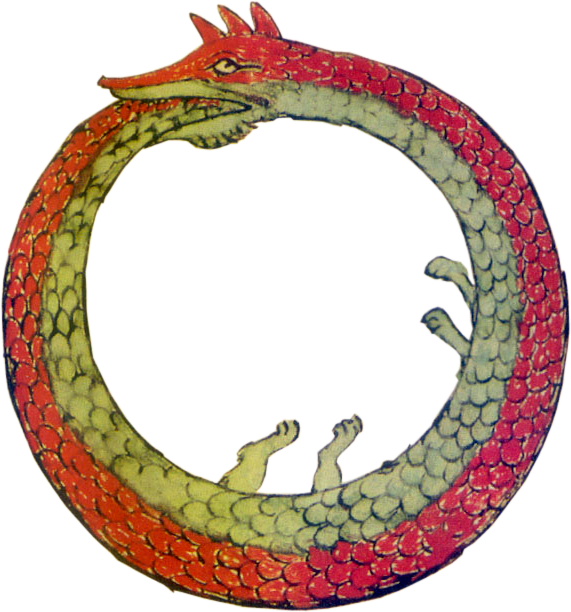
\includegraphics[width=0.4\textwidth]{Ouroboros.png}
        \vfill
\end{center}

\tableofcontents

\section{Introduction}
\subsection*{}
The `infinite snake' is a non-holonomic planar mechanical system:
an infinite chain of rigid segments of unit length, with kinematics
constrained by the requirement that the instantaneous velocity of
a segment's midpoint be parallel to the segment itself.

Geometrically, these constraints define a non-integrable vector distribution $D \subset T\sM$ (a
sub-bundle of the tangent bundle) on the system's configuration space $\sM$ (an infinite-dimensional
manifold). It has rank 2, and is spanned by a distinguished pair of vector fields $X,Y \in \XX(\M)$. 
Their iterated Lie brackets satisfy non-trivial relations, and the main result of this paper is
an \emph{explicit isomorphism} between the Lie subalgebra generated by $X,Y$ in $\XX(\M)$, and
the positively graded ideal of a \emph{twisted loop algebra} of
$\so(2,1)$.
Furthermore, this Lie algebra can also be identified with the \emph{symbol} of $D$ at a generic point,
a fundamental invariant of a non-integrable distribution.

In the remainder of this introductory section, I will sketch the broader context of this work,
state the main results in a precise form, and outline the contents of the article.

\subsection{}
The infinite snake has its origins in a `geometric robots' project proposed by Pawel Nurowski around 2014.
I will briefly explain its two fundamental ideas:
\begin{enumerate}
        \item certain non-integrable distributions can be viewed as sources of rich geometry, 
        \item a large supply of interesting non-integrable distributions is offered
              by simple, toy-like mechanical systems.
\end{enumerate}

Traditionally, non-integrable distributions arise in areas such as \textsc{PDE}s, non-holonomic mechanics,
and control theory. Pursuing their intrinsic properties, one quickly arrives at the problem of local 
equivalence (including auto-equivalence, i.e. symmetry).
That in turn forces one to consider local invariants of a non-integrable distribution, in particular 
its \emph{symbol}:
a bundle of graded Lie algebras, associated with an increasing 
filtration of the tangent bundle induced by the
distribution (possibly after removing a singular subset). 

The filtration $F^\bullet TM$ induced by $D \subset TM$
satisfies $F^0TM=0$, $F^1TM=D$ and is minimal with the property that $[\Gamma(F^iTM), \Gamma(F^jTM)]
\subset \Gamma(F^{i+j}TM)$. There is a smallest $k>0$ such that $F^kTM$ is involutive, and 
we shall assume that actually $F^k TM=TM$ (i.e. the filtration is exhaustive); otherwise,
we would restrict to its leaves. The sequence $(\rk F^i TM)_{1 \le i \le k}$ is called the
\emph{growth vector} of $D$.

Now, the symbol is the associated graded object of $F^\bullet TM$, a graded vector bundle over $M$.
Its fibres have a natural structure of graded nilpotent
Lie algebras, generated in degree one, 
with graded components in degrees $1,\dots,k$ of dimensions encoded by the increments
of the growth vector (padded by zero on the left). 
We may visualise this data as a map from $M$ into the moduli space of such 
Lie algebras. Distributions for which this map is constant are of particular interest: by the
work of Tanaka and others, they allow one to construct a Cartan geometry
over the base manifold. 
Having fixed the isomorphism class of symbol algebras, this construction
can be made functorial, thus reducing the equivalence problem for such
distributions to the equivalence problem for certain
Cartan geometries.

From this point of view geometry is a means to the end of classifying non-integrable distributions,
with further practical applications in mind. The first idea underlying the `geometric robots' project
is to take the opposite view: non-integrable distributions, through the process described above, can be
used to generate geometric structures of much richer nature. For example,
generic rank two distributions in dimension five induce on their underlying fivefold a Cartan geometry
modeled on a homogeneous space for the split real form of the exceptional group $\mathsf{G}_2$, along
with a wealth of associated objects, including a conformal class of signature $(3,2)$.

How then does one produce interesting distributions? Nurowski was inspired by the work of Masato Ishikawa,
exploring certain robotic systems from an engineering perspective, yet revealing remarkably deep geometric
properties. In particular, Ishikawa studied (also experimentally!) planar robots built from rigid elements
(segments or polygons), connected at adjacent vertices by active rotating joints, and possibly equipped
with passive wheels. The condition that the wheels roll without skipping or skidding introduces non-holonomic
constraints, cutting out a non-integrable distribution in the tangent bundle of the robot's configuration space.
One such robot, the \emph{three-segment snake}, gives rise to a generic rank two distribution in dimension five,
and thus to a $\mathsf{G}_2$ Cartan geometry. Another, the \emph{trident snake}, induces a generic rank three
distribution in dimension six, corresponding to an $\mathsf{SO}(4,3)$ Cartan geometry. 
One may easily imagine other `snakes', i.e. planar robots
composed of rigid segments and passive wheels with a no-skidding-or-skipping constraint. These systems have
a combinatorial flavour, but also include continuous parameters, 
namely segment lenghts and wheel positions, giving rise to
families of geometries (perhaps with special, exceptionally symmetric, members). That is the second idea underlying the `geometric robots' project.

\subsection{}\label{subsec:table}
How much can be deduced from a `snake's combinatorial structure? Certainly the dimension of its configuration
space, and the rank of the constraint distribution -- the initial and final entries of the growth vector (assuming the filtration of the tangent bundle is exhaustive). What about the entire growth vector? I was approaching
this question in 2014, attempting to understand what happens as a `snake' is built inductively, by appending
new segments one by one. Arguably the simplest construction of this sort is the one that resembles
an actual snake: a sequence of segments, each attached to the end of the previous one. With each segment
equipped with a wheel in its very middle, these systems are what we'll call $n$-segment snakes (including
the $3$-segment snake mentioned above in relation to $\mathsf{G}_2$).

Here are the growth vector increments (i.e. ranks of graded
components of the symbol) for the first few:
\begin{center}\begin{tabular}{@{}lclllllll@{}}
        $n$ & & \multicolumn{7}{c}{growth vector increments} \\
        \midrule
        $1$ & & $2$ & $1$ \\
        $2$ & & $2$ & $1$ & $1$ \\
        $3$ & & $2$ & $1$ & $2$ \\
        $4$ & & $2$ & $1$ & $2$ & $1$ \\
        $5$ & & $2$ & $1$ & $2$ & $1$ & $1$ \\
        $6$ & & $2$ & $1$ & $2$ & $1$ & $2$ \\
        $7$ & & $2$ & $1$ & $2$ & $1$ & $2$ & $1$ \\
        $8$ & & $2$ & $1$ & $2$ & $1$ & $2$ & $1$ & $1$\\
        $9$ & & $2$ & $1$ & $2$ & $1$ & $2$ & $1$ & $2$ \\
\end{tabular}
\end{center}
The pattern is evident: the growth vector increments are an alternating
sequence of $2$ and $1$, except perhaps for the terminal entry, where
a $1$ can appear instead of $2$. The initial entry is $2$, and that's the rank
of the constraint distribution. The sum of the entries is $n+2$, and that's the
dimension of the configuration space. Explaining this pattern had been the main
motivation behind this paper.

\subsection{}
Let us quickly sketch the connection between Theorem~\ref{thm:main} and the above table
of growth vector increments. We need to consider $n$-segment snakes for $n \in \NN \cup \{\infty\}$.
The $n$-segment snake is described by a configuration space $\sM_n$ together with a distribution
$D_n \subset T\sM_n$. In particular, $\sM_0 \simeq \RR^2$ and $D_0 = T\sM_0$.
We may view each finite snake as a subsystem of the infinite snake,
consisting of the snake's `head', along with a finite number of subsequent segments. Shorter finite
snakes are in turn subsystems of longer finite snakes, so that eventually we have projection maps
\[ \pi^n_{n'} : \sM_n \to \sM_{n'},\quad 0 \le n' \le n \le \infty \]
such that $T\pi^n_{n'} : T\sM_n \to T\sM_{n'}$ maps $D_n$ into $D_{n'}$. 
It turns out that in fact the latter map induces isomorphisms between the fibres of $D_n$ and $D_{n'}$.
Ultimately, taking $n'=0$ we find that $\rk D_n = 2$ for all $n \in \NN \cup \{\infty\}$.

The translation group $\RR^2$ acts on all the $\sM_n$, so that the projections $\pi^n_{n'}$
are equivariant, and the distributions $D_n$ are invariant. In particular, the action trivialises
$T\sM_0 \simeq \sM_0 \times \RR^2$; combining this with isomorphisms $D_n \simeq \pi^{n*}_{n'} D_{n'}$
induced by the projections, we obtain trivialisations $D_n \simeq \sM_n \times \RR^2$. Eqiuvalently, for each 
$n \in \NN \cup \{\infty\}$
we get a map
\[ \RR^2 \to \XX(\sM_n) \]
whose image spans $D_n$ at each point. Letting $\FL(\RR^2)$ denote the free Lie algebra on the vector
space $\RR^2$ (i.e. the free Lie algebra on two generators), the above map extends to a Lie algebra homomorphism
\[ \phi_n : \FL(\RR^2) \to \XX(\sM_n) \]
by the universal property of $\FL$.

The algebra $\FL(\RR^2)$ is naturally graded; we may also view it as filtered, with $F^\ell \FL(\RR^2)$
spanned by elements of degree $\le \ell$. On the other hand, letting $m \in \sM_n$
be a regular point with an open neighbourhood $U \subset \sM_n$
over which $D_n$ induces a well-defined filtration $F^\bullet TU$ by vector sub-bundles,
we may set $F^\ell\XX(U) = \Gamma(F^\ell TU)$. Then the map
\[ \res_U \circ \phi_n : \FL(\RR^2) \to \XX(U) \]
is compatible with the filtrations, and the image of $F^\ell\FL(\RR^2)$
spans $F^\ell TU$ at each point. Thus, via evaluation at $m$, we have a surjective  homomorphism
of \emph{graded} Lie algebras
\[ \phi_{n,m}^{\Symb} : \FL(\RR^2) \to \Symb_m D_n \]
onto the \emph{symbol} of $D_n$ at $m$. 
To understand the latter, we need to control $\ker\phi_{n,m}^{\Symb}$.
So far, we have:
\[ \ker\phi_n \subset \ker \phi_{n,m}^{\Symb}.  \]

In fact, the image of $\phi_n$ is contained in the Lie subalgebra $\XX^{\pr}(\sM_n)$
of \emph{projectable} vector fields
with respect to all the projections $\pi^n_{n'}$, $n'\le n$: these are the vector fields on $\sM_n$
whose action as derivations preserves each subalgebra $\pi^{n*}_{n'}C^\infty(\sM_{n'}) \subset C^\infty(\sM_n)$.
Projection maps $\pi^n_{n'}$ induce well-defined Lie algebra homomorphisms
\[ \pi^n_{n'*} : \XX^{\pr}(\sM_n) \to \XX^{\pr}(\sM_{n'}), \]
and we have by construction that\footnote{
By the way, if the reader is uncomfortable working with the infinite-dimensional
$\sM_\infty \simeq \varprojlim_{n<\infty} \sM_n$, limit of a diagram of spaces (manifolds?),
it is enough accept the more palatable
$\XX^{\pr}(\sM_\infty) \simeq \varprojlim_{n<\infty} \XX^{\pr}(\sM_n)$,
limit of a diagram of Lie algebras.}
\[ \phi_{n'} = \pi^n_{n'*} \phi_n\,\quad 0\le n'\le n \le \infty. \]
Hence $\ker \phi_n \subset\ker\phi_{n'}$ for $n' \le n$, and
in particular
\[ \ker\phi_\infty \subset \ker\phi_n \subset \ker\phi_{n,m}^{\Symb}. \]

Even further, $\phi_n$ does in fact factor through $\XX^{\pr}(\sM_n)^{\RR^2}$, the
subspace of \emph{translation-invariant} projectable vector fields on $\sM_n$ (of course preserved by the $\pi^n_{n'*}$).
Specialising to $n=\infty$ and omitting projectability, let us consider the quotient map
\[ 0 \to \RR^2 \to \XX(\sM_\infty)^{\RR^2}\xrightarrow{q} \XX(\sM_\infty/\RR^2). \]
Theorem~\ref{thm:main} states that the image of $q \circ \phi_\infty$ is isomorphic to
the graded Lie algebra
\[ \fL_+ = \bigoplus_{i>0} \fL_i,\quad \fL_{2i} \simeq \so(2),\quad \fL_{2i+1} \simeq \RR^2 \]
with Lie brackets induced by the Cartan decomposition 
\[ \so(1,2) = \so(2) \oplus \RR^2. \]
We may restate it as follows.
\begin{thm*}
There is a commutative diagram of Lie algebra homomorphisms
\[\begin{tikzcd}
        \FL(\RR^2) \arrow[d, "\psi", two heads] \arrow[r,"\phi_\infty"] & \XX(\sM_\infty)^{\RR^2} \arrow[d,"q",two heads] \\
        \fL_+ \arrow[r,"\iota",rightarrowtail] & \XX(\sM_\infty/\RR^2) 
\end{tikzcd}\]
where $\psi$ is a graded surjection induced by the identification $\fL_1=\RR^2$ and the universal property of $\FL$,
while $\iota$ is an injection. 
\end{thm*}

In particular, $\ker \phi_\infty \subseteq \ker(q \circ \phi_\infty) = \ker\psi$. In fact, it turns out that
the inclusion is an equality, so that eventually
\[ \ker\psi = \ker\phi_\infty \subset \ker\phi_{n,m}^{\Symb}. \]
Put differently, the symbol of $D_n$ at a general point $m \in \sM_n$
is a \emph{graded quotient} of $\fL_+$. Now the puzzle is essentially reduced to the 
following observation:
\begin{prop*} For each $n \in \NN$, there is, up to isomorphism, precisely one $(n+2)$-dimensional graded quotient 
        Lie algebra of $\fL_+$ generated in degree $1$. The ranks of its graded components follow the
        pattern of the table in Subsection~\ref{subsec:table}.
\end{prop*}

\subsection{}
The proof of Theorem~\ref{thm:main} is, ultimately, computational. The calculation is however greatly
simplified by exploiting \emph{symmetries} of the main system of interest: the infinite snake. We've already
employed \emph{translational} symmtery, working with vector fields on the reduced configuration space, which
we'll now denote simply by $M=\sM_\infty /\RR^2$. We'll also write $\xi = q \circ\phi_\infty$.
Of course, the original system enjoyed full \emph{Euclidean}
symmetry, whence we're still left with the rotation group $\O(2)$ acting on $M$, so that the
homomorphism
\[ \xi : \FL(\RR^2) \to \XX(M) \]
becomes $\O(2)$-equivariant with respect to the natural induced actions on the domain and codomain.

It is natural to diagonalise the $\SO(2)$-actions. This requires
complexifying the above situation:
\[ \xi : \FL(\CC^2) \to \XX_\CC(M) = \CC \otimes \XX(M)\]
where we extend $\xi$ to a complex-linear map. 
Let $v^\pm = e_1 \pm ie_2$ be an isotropic basis of $\CC^2$,
with a suitable generator of $\so(2,\CC)$ acting as $v^\pm\mapsto\pm v^\pm$.
We are interested in the Lie subalgebra 
generated by
\[ \zeta^\pm = \xi(v^\pm) \in \XX_\CC(M). \]
These turn out to satisfy certain remarkable identities.

There's a further semi-symmetry we haven't yet exploited: the tail of an infinite snake
is itself an infinite snake -- and it behaves as such. That is, the resulting map
$\tail:\sM_\infty \to \sM_\infty$ sends $D_\infty \subset T\sM_\infty$ to itself.
Observe that the data corresponding to $\tail$ at the finite $n$ level
is a map $\sM_n \to \sM_{n-1}$; this only becomes a self-map at $n=\infty$.
Of course, $\tail$ is not invertible -- hence the prefix \emph{semi}.\footnote{One could
go further and consider doubly infinite snakes, with $\tail$ becoming an honest symmetry.}

Much of Sections \ref{sec:deriving} and \ref{sec:abstracting} is devoted to 
working out how the tail map interacts with $\xi$, and thus $\zeta^\pm$. While this is
not difficult, and quite entertaining to see intuitively, some care has to be taken to
write down correct equations for $\xi$ and $\zeta^\pm$. 
In short, one considers a \emph{twist} $\ttl:M \to M$ of the tail map descended to $M$,
along with the head map $\hd : M \to \TT$: these define an isomorphism
\[ \langle \hd,\ttl\rangle : M \xrightarrow{\simeq} \TT \times M. \]
Using its inverse, we consider the pair of injective homomorphisms
\[ \XX_\CC(\TT) \xrightarrow{\iota} \XX_\CC(M) \xleftarrow{\sigma} \XX_\CC(M) \]
of Lie algebras. In particular, the `shift operator'
$\sigma$ sends an infinitesimal motion of the infinte snake,
now viewed as the tail of another infinite snake, to
an infinitesimal motion of the latter, keeping the head immobile. 
Now, we have the relation:
\begin{equation}\label{eq:rec-rel-first}
        \zeta^+ = z^2\partial_z + z\sigma\left(\zeta^+ + z\partial_z \right) 
\end{equation}
where $z \in C^\infty(\TT, \CC)$ is the standard complex coordinate
on the torus, and we've omitted the maps $\hd^* : C^\infty(\TT,\CC) \to C^\infty(M,\CC)$
and $\iota : \XX_\CC(\TT) \to \XX_\CC(M)$ from notation.

Here's a number of observations regarding \eqref{eq:rec-rel-first}.
\begin{enumerate}
        \item 
                The operator $1 - z\sigma : \XX_\CC(M)\to\XX_\CC(M)$ is invertible,
                so that \eqref{eq:rec-rel-first} determines $\zeta^+$ uniquely.
        \item 
                There is a reflection in $\O(2)$ inducing involutions
                on $\XX_\CC(M)$ and related spaces, denoted by $\tau$,
                such that $\tau\sigma=\sigma\tau$, $\tau z = z^{-1}\tau$
                as operators on $\XX_\CC(M)$, and
                $\zeta^- = \tau\zeta^+$. Hence \eqref{eq:rec-rel-first} determines $\zeta^-$ as well.
        \item 
                The vector fields $z^2\partial_z$, $z\partial_z$ and $\tau(z^2\partial_z) = \partial_z$,
                identified with their images under $\iota$,
                form a Lie algebra isomorphic to $\sl(2,\CC)$, a complexification of the
                $\so(1,2)$ giving rise to the loop algebra $\fL_+$ eventually controlling the 
                entire situation. This is a first glimpse of the role of $\so(1,2)$ in the infinite
                snake's kinematics.
\end{enumerate}
In light of the latter observation, one may contemplate three factors in the infinite snake's generalised
symmetries: obvious Euclidean symmetry, `shift' semi-symmetry, and `hidden' $\so(1,2)$. 

One may view \eqref{eq:rec-rel-first}
as constructing an object over the infinite-dimensional space $M$
in terms of finite-dimensional data -- a pair of elements of $\sl(2,\CC)$ embedded in $\XX_\CC(M)$.
That is the `taming' of the snake's infinite aspect by means of the shift semi-symmetry and associated (co)recursion 
(cf. the picture of Ouroboros eating its tail on the title page).
The strategy for proving Theorem~\ref{thm:main} is now easy to guess: we seek relations analogous
to \eqref{eq:rec-rel-first} satisfied by iterated Lie brackets of $\zeta^\pm$, and use these to
determine $\ker\xi \subset \FL(\CC^2)$.

\subsection{}
Section \ref{sec:deriving} constructs the reduced configuration space $M$ along
with the map $\RR^2 \to \XX(M)$, and derives an identity relating the latter with
the tail map. Section \ref{sec:abstracting} passes to the complexification and
then to a further abstract setting, defined by algebraic relations between
$\sigma$, $z$, etc. Theorem~\ref{thm:main} is reduced to its algebraic analogue, Theorem~\ref{thm:algebraic}.
The latter is proved in Section \ref{sec:proving}. Finally, Section \ref{sec:final} fills in
some details regarding the symbols of finite snakes, and discusses several other aspects of
our result.

\subsection*{Acknowledgements}
\endinput

\section{Deriving snake kinematics.}
\label{sec:deriving}
\subsection*{}
In what follows, we will work with certain infinite-dimensional manifolds 
in a rather synthetic manner. Formally, this involves an extension of the
usual category of $\Cinf$ finite-dimensional manifolds and $\Cinf$ maps, with
suitable properties. There are many possible choices of such a category,\footnote{
In particular, any well-adapted model of Synthetic Differential Geometry
(see Moerdijk and Reyes, \textit{Models for Smooth Infinitesimal Analysis}). In fact,
it is enough to have limits of sequences of locally trivial fibrations of 
finite-dimensional manifolds, and then to work with Lie algebras of projectable 
vector fields. Indeed, one could express the entire construction in terms of 
sequences of finite-dimensional manifolds, at the cost of index bookkeeping 
completely obscuring the intuitive geometric picture. 
}
and the resulting algebraic object we're interested in -- the Lie algebra of 
vector fields generated by lifts of Euclidean translations to the snake's 
reduced configuration space -- is invariant. Thus, on one hand, we will 
proceed with its construction assuming the spaces and maps make sense in
a suitable category; on the other hand, in section \ref{sec:abstracting} we'll reformulate the
Main Theorem in a purely algebraic setting; section \ref{sec:proving} of the paper
is devoted to proving this purely algebraic formulation.


\subsection{}
The snake lives in a Euclidean plane $\E$. Its basic building block
is a single segment. The configuration of a single segment is
parameterised by a pair of points at unit distance. These pairs
form a double circle fibration:
\[
    \pr_1, \pr_2 : \S\rightrightarrows \E;\quad \S = \{ (p,q)\ |\ |p-q|=1 \} \subset \E \times \E.
\]
The motion of the segment is uniquely determined by
the motion of one of its endpoints. Correspondingly, there
is a rank two distribution
\[
    \D_\S \subset T\S
\]
fitting into a commutative diagram
\[
\begin{tikzcd}
           &  \D_\S 
           \arrow[ld, "\pr_{1*}" left]
           \arrow[rd, "\pr_{2*}" right]
           & \\
        \pr_1^* T\E  
           \arrow[rr, "\Phi"]
           & &   \pr_2^* T\E
\end{tikzcd}
\]
of isomorphisms of vector bundles over $\S$. Evaluating $\Phi$ at $s=(p,q) \in \S$,
we have that 
\[
    \Phi_s : T_p \E \to T_q \E
\] 
is a \emph{reflection} in the line $\overline{pq}$, followed by parallel transport
(this can be taken as an axiom).

\subsection{}
Now, the configuration space of an infinite snake is an infinite
fibre product
\[
    \M = \S \times_\E \S \times_\E \S \times_\E \cdots
\]
where $\S$ is viewed as fibred over $\E$ using $\pr_1$ on the left and $\pr_2$ 
on the right. It follows that $\M$ carries a rank two distribution
\[
\begin{tikzcd}
        \D \arrow[d,hookrightarrow] \arrow[r,equal] & \D_\S \times_{T\E} D_\S \times_{T\E} \cdots \arrow[d,hookrightarrow] \\
        T\M \arrow[r,equal] & T\S  \times_{T\E} T\S  \times_{T\E}\cdots
\end{tikzcd}
\]
Consider the projections
\[
     \S  \xleftarrow{\head} \M  \xrightarrow{\tail}  \M               
\]
\begin{eqnarray*}
        \head(s_1,s_2,s_3,\dots) &=& s_1 \\
        \tail(s_1,s_2,s_3,\dots) &=& (s_2,s_3,\dots)
\end{eqnarray*}
together with
\[      \nose = \pr_1 \circ \head : \M \to \E \]
\[      \neck = \pr_2 \circ \head : \M \to \E \]
so that
\[      \neck = \nose \circ \tail. \]
Note that we get a coinductive\footnote{
\emph{Coinductive,} because it exhibits $\M$ as a \emph{final coalgebra}
for the endofunctor $\S \times_\E -$ on the category of locally trivial fibre 
bundles over $\E$
}
description of $\M$:
\[
        \langle \head, \tail \rangle : \M \xrightarrow{\simeq} \S \times_\E \M
\]
Now, in particular the map
\[
    \nose_* : T\M \to \nose^* T\E
\]
restricts to an \emph{isomorphism} on the rank 2 distribution $\D \subset T\M$.

\subsection{}
Consider the translation action of $\RR^2$ on $\E$, and the induced actions
on $\S$, $\M$, their tangent bundles and so on. Note that the distributions
$\D_\S$ and $\D$ are translation invariant, and the maps $\head$, $\tail$, etc. 
defined above are equivariant. We may consider the reduced configuration
space 
\[
   \Mr = \M / \RR^2, 
\]
along with its coinductive description
\[
        \langle\hd, \tl\rangle : \Mr \xrightarrow{\simeq} \TT \times \Mr 
\]
where $\TT\subset\RR^2$ is the unit circle, identified with $\S/\RR^2$. This in particular
exhibits $\Mr$ as an infinite torus, parameterising orientations of the
infinite snake while forgetting the position of its nose.

\subsection{}
Let $\RR^2 \to \XX(\E)$ be the infinitesimal action map, an isomorphism onto
the space of translation-invariant vector fields. Inverting the 
isomorphism
\[
    \nose_* : \D \to \nose^* T\E
\]
gives rise to a map of vector fields
\[
    \nabla : \XX(\E) \to \Gamma(\M,\D),\quad  (T_m \nose)(\nabla\upsilon) = \upsilon_{\nose m}
\]
restricting to a lifting of translation-invariant fields. Following
with projection $\M \to \Mr$, we have a map
\[
        \xi : \RR^2 \to \XX(\E)^{\RR^2} \xrightarrow{\nabla} \Gamma(\M,\D)^{\RR^2} \to \XX(\M)^{\RR^2} \to
        \XX(\Mr).
\]
The group $\O(2)$ acts on $\RR^2$, $\TT$ as well as $\E$, $\S$, $\M$, etc. so that all 
the relevant maps are equivariant. In particular, the action
descends to $\Mr$ so that $\xi$ is $\O(2)$-equivariant.

\begin{thm}\label{thm:main}
       Consider $G = \SO(1,2)$, with maximal compact subgroup
$\O(2) \subset G$, and a Cartan involution $\theta$ acting on the Lie algebra $\fg$
with even eigenspace $\so(2)$ and odd eigenspace $\RR^2$ (as $\O(2)$-modules).
Let 
\[
    \L_+ = \{ f(t) \in t \fg[t]\ |\ f(-t) = \theta f(t) \} = \bigoplus_{i>0} \L_i
\]
be the positive part of the corresponding twisted loop algebra,
with $\L_{2i} \simeq \so(2)$, $\L_{2i+1} \simeq \RR^2$. Then there exists an 
$\O(2)$-equivariant Lie algebra homomorphism 
\[
    \xi^+ : \L_+ \to \XX(\Mr) 
\]
such that the following diagram commutes:
\[\begin{tikzcd}
        \L_1 \arrow[r,hookrightarrow]\arrow[d,"\simeq"] & \L_+ \arrow[d,"\xi^+"]\\
  %≃ ↓    ↓ ξ⁺
        \RR^2 \arrow[r,"\xi"] & \XX(\Mr).
\end{tikzcd}\]
Furthermore, $\xi^+$ is injective, and thus an isomorphism onto
the sub-algebra generated by the image of $\xi$ in $\XX(\Mr)$.
\end{thm}

\subsection{}
Consider the 2:1 map 
\[
        \gamma : \TT \to \O(2)
\]
parameterising reflections so that $\gamma_u u = u$ for all $u\in\TT$. We may
view $\gamma$ as a translation quotient of $\Phi$. 
\begin{lem}\label{lem:xi-rec}
$\forall m \in \Mr, v \in \RR^2.\ (T_m \tl)\xi(v)_m = \xi(\gamma_{\hd m} v)_{\tl m}.$
\end{lem}
\begin{proof}
Identifying $\RR^2$ with $\XX(\E)^{\RR^2}$, let $\upsilon=\nabla v$, and let $m' \in\M$ be a 
lift of $m \in\Mr$. Then
\[
        (T_{m'} \head)(\upsilon_{m'}) \in \D_{\S,\head m'}
\]
and thus
\begin{eqnarray*}
        (T_{\tail m'}\nose)(T_{m'} \tail)(\upsilon_{m'}) &=& (T_{m'} \neck)(\upsilon_{m'}) \\
                                                         &=& \Phi_{\head m'} (T_{m'} \nose)(\upsilon_{m'}) \\
                                                         &=& \Phi_{\head m'} v
\end{eqnarray*}
by commutativity of the diagram defining $\D_\S$. Since 
\[
    \tail_* : \D \to \tail^* \D,\quad
    \nose_* : \D \to \nose^* T\E 
\]
are isomorphisms over $M$, it follows that 
\[
        (T_{m'} \tail)(\nabla v)_{m'} = \nabla(\gamma_{\hd m} v)_{\tail m'},
\] 
descending along $\M\to\Mr$ to the desired identity at $m\in\Mr$.
\end{proof}
The lemma is equivalent to commutativity of the following diagram
\[\begin{tikzcd}
        \Mr\times\RR^2 \arrow[r,"\hd^*\gamma"]\arrow[d,"\xi"] 
        &  \Mr\times\RR^2 \arrow[r,"\mathrm{triv.}"] & \tl^* (\Mr\times\RR^2) 
        \arrow[d,"\tl^*\xi"] \\
        T\Mr \arrow[rr,"\tl_*"] & &  \tl^* T\Mr
\end{tikzcd}\]
of vector bundles over $\Mr$, where $\hd^*\gamma$ is an endomorphism of the
trivial $\RR^2$-bundle induced by the composite $\gamma\circ\hd : \Mr\to\O(2)$,
and we identify $\xi$ with a bundle morphism $\Mr\times\RR^2\to T\Mr$.

\subsection{}
Lemma \ref{lem:xi-rec} provides a corecursive description of $\xi$, with respect to
the coinductive description of $\Mr$ in terms of $\hd$, $\tl$. It expresses 
the tail part of $\xi$ as a twist of $\xi$ by $\hd^* \gamma$. Our strategy for proving
the main theorem will be to use similar corecursive descriptions of
iterated Lie brackets of vector fields in the image of $\xi$. More succintly,
we seek recursion relations for the Lie algebra homomorphism 
\[
  \txi : \FL(\RR^2) \to \XX(\Mr)
\]
from the free Lie algebra on $\RR^2\simeq\L_1$, in order to show that it descends
along the quotient map $\FL(\L_1) \to\L_+$. 

This task will be simplified if we twist the tail map $\tl$ by a reflection:
then the recursion relation will be expressed in terms of rotations only,
and these can be simultaneously diagonalised upon complexification. To this
end, let
\[
  \rho : \TT \to \SO(2)
\]
be the 1:1 parameterisation of rotations, so that $\rho_u(e_1)=u$. Consider the
\emph{twisted tail map}
\[
        \ttl : \Mr\to\Mr,\quad  \ttl(m) = \gamma_{e_1} \rho_{\hd(m)}^{-1} \tl(m).
\]
Note that it still leads to a coinductive description
\[
        \langle\hd, \ttl\rangle : \Mr \xrightarrow{\simeq} \TT\times\Mr.
\]
Intuitively, if we used $\langle\hd,\tl\rangle$ iteratively to identify $\Mr$ with an intinite
torus, we'd be parameterising the snake's oriention in terms of the angle each
segment makes with $e_1$. On the other hand, if we used $\langle\hd,\ttl\rangle$, we would be
using the angle the head makes with $e_1$, and then the angle each subsequent segment
makes with the previous one, measured with alternating orientations. For instance,
the point on the infinite torus with all angular coordinates equal corresponds to:
a straight-line snake in the former case; and a zig-zag snake in the latter (Fig.~\ref{fig:param}). 

\begin{figure} % TODO: redo in tikz
\begin{verbatim}
        a)   /     b)   _   
            /         _/
           /         /
          /               
\end{verbatim}
\caption{
        $(\frac{\pi}{4},\frac{\pi}{4},\dots) \in \TT^\infty\simeq\Mr$
        using (a) $\langle\hd,\tl\rangle$ and (b) $\langle\hd,\ttl\rangle$.
\label{fig:param}}
\end{figure}

\begin{lem}\label{lem:ttl-refl}
        $\ttl\circ\gamma_{e_1} = \gamma_{e_1}\circ\ttl$
\end{lem}
\begin{proof}
By $\O(2)$-equivariance of the head map $\hd$ and untwisted tail map $\tl$,
\begin{eqnarray*}
        \ttl(\gamma_{e_1}m) &=& \gamma_{e_1} \rho_{\gamma_{e_1} \hd(m)}^{-1} \gamma_{e_1} \tl(m) \\
                            &=& \rho_{\hd(m)}^{-1} \tl(m) \\
                            &=& \gamma_{e_1} \ttl(m)
 \end{eqnarray*}
for $m\in\Mr$.
\end{proof}

\subsection{}
Consider the action map
\[  \act \circ \rho : \TT  \to \Aut(\Mr), \]
its differential
\[  \alpha : T\TT \to \XX(\Mr) \]
and the associated evaluation map
\[  \alpha_\bullet : \Mr\times T\TT \to T\Mr. \]
\begin{lem}\label{lem:ttl-diff}
$\forall m\in \Mr, v \in T_m\Mr.\
(T_m \ttl)(v) = \gamma_{e_1} \rho_{\hd(m)}^{-1} \cdot [ (T_m \tl)(v) - \alpha_{\tl m} (T_m \hd)(v) ]$.
\end{lem}                               
Observe that the right hand side involves an element of $\O(2)$ acting on the bracketed expression
$[\cdots] \in T_{\tl m} \Mr$,
and belongs to $T_{\ttl m}\Mr$. 

\begin{proof} This is an immediate application of the chain rule to $\ttl$, where we note
        that $-\alpha$ is the differential of $\act \circ \rho^{-1}$.
\end{proof}


This result may be understood intuitively as follows. Consider a snake whose nose
is located at the origin of a Cartesian frame with unit vectors $e_1,e_2$. The map $\tl$
may be viewed as cutting off the head of the snake, and moving the frame by translation
to the new nose. On the other hand, the map $\ttl$ constructs a \emph{new} frame with origin at
the new nose: its orientation is opposite to the previous one, and its first axis is
in the direction of the severed head. Thus, given an infinitesimal motion of the snake,
its images under $\tl$ and $\ttl$, besides being expressed in different frames, differ by
a term arising from an infinitesimal rotation of the frame itself. The latter term
is the $\alpha_{\tl m} (T_m \hd)(v)$ in the Lemma.

\subsection{}
Let $\omega = e_1\wedge e_2$, viewed interchangeably as an element of $\Lambda^2\RR^2$, its dual, or $\so(2)$;
in the latter case, $\langle\omega(u),v\rangle = \omega(u,v)$ for $u,v \in\RR^2$. Write $\tom\in\XX(\Mr)$ for the 
corresponding infinitesimal action. 

\begin{lem}\label{lem:xi-rec-twisted}
$\forall m \in \Mr, v \in \RR^2.\ (T_m \ttl)(\xi(v)_m) = [ \xi(\rho_{hd(m)}^{-1} v) - \omega(\hd m, v) \tom ]_{\ttl m}$.
\end{lem}
\begin{proof}
Combining Lemmas \ref{lem:ttl-diff} and \ref{lem:xi-rec-twisted}, we have:
\begin{eqnarray*}
        (T_m \ttl)\xi(v)_m &=& \gamma_{e_1} \rho_{\hd(m)}^{-1} \cdot [ \xi(\gamma_{\hd m} v)_{\tl m} - \alpha_{\tl m} (T_m \hd)(\xi(v)_m) ] \\
                           &=& \xi(\rho_{\hd(m)}^{-1} v)_{\ttl m} + \alpha_{\ttl m} (T_m \hd)(\xi(v)_m) 
\end{eqnarray*}
for all $m \in\Mr$, $v\in\RR^2$, where we used $\gamma_u = \rho_u \gamma_{e_1} \rho_u^{-1}$. Now, using
\[
        (T_m \hd) \xi(v)_m = \frac{\gamma_{\hd m}-1}{2} v
\]
and
\[
  (T_u \rho)(v) = \omega(u,v)\omega 
\]
we have
\[
  \alpha((T_m \hd)(\xi(v)_m)) = \omega(\hd m, -v) \tom
\]
and the claim follows. 
\end{proof}
\section{Abstracting the algebra.}
\label{sec:abstracting}
\subsection*{}
Recall that the point of `twisting' the snake's tail was to have a
recursion relation (namely that of Lemma \ref{lem:xi-rec-twisted})
involving rotations rather than reflections. The next step is then
to complexify $\XX(\Mr)$, so that the action of $\SO(2)$ becomes
diagonalisable, simplifying the relation. Furthermore, we'll replace
the `geometric' formula of Lemma \ref{lem:xi-rec-twisted}, expressed
in terms of head and tail maps, with an `algebraic' one, involving
certain operators on $\XC(\Mr)$. Then, the structure on $\XC(\Mr)$ necessary to
express the recursion relation becomes simple enough to be abstracted in the (purely algebraic)
notion of an \emph{ambient module} (Definition \ref{defn:ambient}). We will 
rephrase Theorem \ref{thm:main} as a statement about ambient modules (Theorem \ref{thm:algebraic}), and prove it
in this context, improving clarity and escaping any uneasiness about the infinite-dimensional
geometric setting.


\subsection{}
Define the Lie algebra homomorphism
\[
  \sigma : \XX(\Mr) \to \XX(\Mr)
\]
by
\[
  \hd_* (\sigma\upsilon) = 0, \quad \ttl_* (\sigma\upsilon) = \ttl^* \upsilon
\]
for all $\upsilon\in\XX(\Mr)$. This is a `shift map', sending
an infinitesimal motion of the snake, to that same
motion applied to the (twisted) tail, with head immobile.

Complexify everything, and introduce the notation
\[
        z : \Mr\to\CC,\quad     z(m) = \langle e_1+ie_2, \hd m \rangle
\]
\[
        \partial_z \in \XC(\Mr), \quad \partial_z z = 1, \quad \ttl_* \partial_z = 0
\]
where $\langle-,-\rangle$ is the complex bilinear extension of the usual
scalar product on $\RR^2$.

That is, $z$ is the usual unimodular complex coordinate
on $\TT$, pulled back by $\hd$ to $\Mr$, while $\partial_z$ is the corresponding
complex vector field on $\TT$, realised as an infinitesimal motion
of the head, with (twisted) tail immobile.

Let
\[
    \zeta^\pm = \xi(e_1\pm ie_2) \in \XC(\Mr).
\]
\begin{prop}\label{prop:zeta-rec}
 $\zeta^\pm = z^{\pm1} [ \pm z \partial_z + \sigma (\zeta^\pm\pm z \partial_z) ]$.
\end{prop}
\begin{proof}
Let $v^\pm= e_1\pm ie_2$. For all $u\in\TT$ we claim:
\begin{enumerate}
        \item[i.] $\rho_u v^\pm  = w(u)^{\mp1} v^\pm $
        \item[ii.] $\omega(u,v^\pm) = \pm i w(u)^{\pm1} $
        \item[iii.] $\omega\in\so(2)$ acts on $\TT$ as $iw \partial_w$
\end{enumerate}
where $w(u) =\langle v^+,u\rangle$. Indeed, letting $u = (\cos\phi,\sin\phi)$,
we have \[
        w(u) = e^{i\phi},\quad
\rho_u e_1=u,\quad \rho_u e_2 = (-\sin\phi,\cos\phi),
\]
so that
\[
    \rho_u v^\pm = (e^{\mp i\phi}, \pm i e^{\mp i\phi}) = w^{\mp 1} v^\pm.
\]
Also, $\omega(u,v^\pm)= \pm i e^{\pm i\phi} = \pm i w^{\pm1}$. Lastly, $dw = i w d\phi$ so that
$\partial_\phi = iw \partial_w$.

Now, in $\XC(\Mr)$, we claim that
\begin{enumerate}
        \item[iv.] $\tom = iz \partial_z.$
\end{enumerate}
Indeed, $\ttl_* \tom = 0$ by Lemma \ref{lem:ttl-diff} and $\hd_* \tom = iw \partial_w$ by (iii).

Let us rewrite Lemma \ref{lem:xi-rec-twisted} in the above notation: for all
$m\in\Mr$, $v\in\CC^2$,
\begin{eqnarray*}
        (T_m \ttl) \xi(v^\pm)_m &=& z^{\pm1}(m) [ \xi(v^\pm) \mp i \tom ]_{\ttl m} \\
        (T_m \ttl) \zeta^\pm_m  &=& z^{\pm1}(m) [ \zeta^\pm \pm z \partial_z ]_{\ttl m}.
\end{eqnarray*}
On the other hand,
\begin{eqnarray*}
        (T_m \hd) \xi(v^\pm)_m  &=& \omega(\hd m, -v^\pm) \partial_\phi  \\
        (T_m \hd) \zeta^\pm_m   &=& \pm w(\hd m)^{1\pm1} \partial_w
\end{eqnarray*}
where $w = e^{i\phi} : \TT \to \CC$ as before. Finally, recalling $z = \hd^* w$ along
with $\ttl_*\partial_z=0$ and $\hd_* \circ\sigma = 0$, we have 
\begin{eqnarray*}
        \zeta^\pm &=& \pm z^{1\pm1} \partial_z + z^{\pm1} \sigma ( \zeta^\pm \pm z \partial_z )\\
        &=& z^{\pm1} [ \pm z \partial_z + \sigma (\zeta^\pm \pm z \partial_z) ]. 
\end{eqnarray*}
\end{proof}

\subsection{}
\begin{defn}\label{defn:ambient}
        An \emph{ambient module} is a complex Lie algebra $\Om$ 
together with the following structure:
\begin{center}\begin{tabular}{@{} l l @{}}
\toprule
        elements & $\e, \h, \f \in \Om$ \\
        maps  &     $\tau, \sigma, z : \Om\to\Om$ \\
\midrule
properties \\
\midrule
        \sltwo & $\e,\h,\f$ are linearly independent and 
   $[\h,\e]=\e$, $[\h,\f]=-\f$, $[\f,\e]=2\h$ \\
        \flip & $\tau$ is an involutive Lie algebra  automorphism \\
        \shift & $\sigma$ is an injective  Lie algebra  endomorphism \\
        \twist & $z$ is an invertible vector space endomorphism,
         transcendental over $\CC$ \\
 \midrule\
relations \\
\midrule
        \flip-\sltwo & $\tau \e = -\f$, $\tau \f = -\e$, $\tau \h = -\h$  \\
        \flip-\twist & $\tau\circ z = z^{-1} \circ\tau$ \\
        \flip-\shift & $\tau\circ\sigma=\sigma\circ\tau$ \\
        \shift-\twist & $\forall\varphi\in\CC[z,z^{-1}], x\in\Om.\ [\ad_{\varphi\sigma x}, z] = 0$ \\
        \shift-\sltwo & $\forall\varphi\in\CC[z,z^{-1}], x\in\{\e,\h,\f\}.\ \ad_{\varphi x} \circ \sigma = 0$ \\
        \twist-\sltwo & $\forall\varphi\in\CC[z,z^{-1}], x\in\{\e,\h,\f\}.\ [\ad_{\varphi x}, z] = \varphi z^{1+\lambda(x)}$
        \\
\bottomrule
\end{tabular}\end{center}
where $\lambda(\e)=1$, $\lambda(\h)=0$, $\lambda(\f)=-1$, and by transcendence of $z$ we 
identify the abstract Laurent algebra $\CC[z,z^{-1}]$ with the subalgebra
generated by $z$ and its inverse in $\End_{\CC}\Om$ (vector space endomorphisms).
\end{defn}

Note that an ambient module is simultaneously a module for the
Laurent algebra $\CC[z,z^{-1}]$, and for the Lie algebra $\sl_2(\CC) \simeq \CC\langle \e,\h,\f\rangle$
(where our $\h$ is half of the usual one!). These two structures
are compatible with respect to the usual action of $\sl_2(\CC)$ on Laurent
polynomials: $\e$ as $z^2 \partial_z$, $\h$ as $z\partial_z$, $\f$ as $\partial_z$. Furthermore, the 
involution $\tau$ is compatible with an involution on the Laurent 
algebra sending $z$ to $z^{-1}$. Finally, relations with the shift map 
mean that $\sigma\Om$ commutes with $\CC[z,z^{-1}]\cdot\sl_2(\CC)$, while the adjoint action
of $\CC[z,z^{-1}]\cdot\sigma\Om$ on $\Om$ is $\CC[z,z^{-1}]$-linear in its passive argument. 

\begin{lem}\label{lem:snake-ambient}
       $\XC(\Mr)$ has the structure of an ambient module as suggested
by notation, with $\e=z^2\partial_z$, $\h=z\partial_z$, $\f=\partial_z$, and with $\tau$ induced by the
action of $\gamma_{e_1} \in \O(2)$.
\end{lem}
\begin{proof}
        Note that $\gamma_{e_1}^* z = z^{-1}$. 
        Then relations \flip-\sltwo{} and \flip-\twist{}
        follow immediately. Next, \flip-\shift{} is a consequence of Lemma \ref{lem:ttl-refl}, while
        \shift-\twist{} and \shift-\sltwo{} hold because $\hd_* \circ\sigma=0$ and $\ttl_*\partial_z = 0$,
        respectively. Finally, \twist-\sltwo{} follows by letting $\e,\h,\f$ as defined in terms
of $\partial_z$ act on $z$.
\end{proof}

We will consider this ambient module structure on $\XC(\Mr)$ as canonical.

\begin{defn}\label{defn:serpentine}
        An element $\zeta$ of an ambient module $\Om$ is called \emph{serpentine}
if it satisfies $\zeta = \e + z \sigma (\zeta + \h)$.
\end{defn}

Note that a serpentine element is non-zero: for if zero were serpentine,
we would have $0=z^{-2}[\e,0]=z^{-2}[\e,\e+z\sigma\h]=\sigma\h$, contradicting injectivity of $\sigma$. 
We will refer to the $\tau$-invariant Lie subalgebra generated by a serpentine element
as a \emph{serpentine subalgebra.}

\begin{lem}\label{lem:snake-serpentine}
        $\zeta^+$ is serpentine in $\XC(\Mr)$, and $\zeta^-=\tau\zeta^+$.
\end{lem}

\begin{proof}
        By Prop.~\ref{prop:zeta-rec}, we have
\[
        \zeta^+ = z^2 \partial_z + z \sigma (\zeta^+ + z \partial_z) = \e + z \sigma (\zeta^+ + \h)
\]
so that $\zeta^+$ is serpentine. Furthermore, since $\xi$ is $\O(2)$-equivariant,
it follows that
\[
        \zeta^- = \xi(v^-) = \xi(\gamma_{e_1}v^+) = \gamma_{e_1}\xi(v^+) = \tau\zeta^+.     
\]
\end{proof}

\subsection{}
\begin{defn}\label{defn:complete} A \emph{$\sigma$-filtration} on an ambient module $\Om$ is a
        decreasing filtration $F^\bullet\Om$ by $\CC[z,z^{-1}]$-submodules such that:
\begin{enumerate}
        \item  $F^0\Om=\Om$,
        \item  $\sl_2(\CC)\to\Om/F^1\Om$ is injective,
        \item  $\sigma F^k \Om \subset F^{k+1} \Om$ for all $k\ge0$.
\end{enumerate}
We say that $\Om$ is \emph{separated} (respectively \emph{complete}) if it
admits a $\sigma$-filtration such that the natural map
\[
    \Om \to \varprojlim_k \Om/F^k\Om
\]
is injective (respectively an isomorphism).
\end{defn}

\begin{lem}
Let $\Om$ be an ambient module. If $\Om$ is separated (respectively
complete), it has at most one (respectively exactly one) serpentine
element.
\end{lem}

\begin{proof}
Let $F^\bullet\Om$ be the $\sigma$-filtration exhibiting $\Om$ as an separated ambient
module. Then two serpentine elements differ by an element of 
\[
   \bigcap_k F^k\Om=0.
\]
Furthermore if $\Om$ is complete, the operator $1 - z \sigma : \Om\to\Om$ is invertible
and
\[
        \zeta = (1 - z \sigma)^{-1} (\e + z \sigma \h)
\]
is serpentine.
\end{proof}

\begin{lem} $\XC(\Mr)$ is a complete ambient module.\end{lem}
\begin{proof}
Write $\Om = \XC(\Mr)$. Recalling $\M = \S\times_\E \S\times_\E\cdots$ and passing to
the quotient by the translation group, we have $\Mr = \TT \times \TT \times \cdots$ with
factor projections
\[
        \seg_k = \hd \circ \tl \circ\cdots \circ \tl : \Mr\to\TT\quad   \textrm{($k-1$ compositions)}.
\]
Define a decreasing filtration $F^\bullet T\Mr$ by $F^k T\Mr = \bigcap_{1 \le l\le k} \ker T\seg_l$.
By construction, the natural map 
\[
    T\Mr \to \varprojlim_k T\Mr / F^k T\Mr
\]
is an isomorphism (of vector bundles over $\Mr$). The same then holds for
the twisted version 
\[
    T\Mr \to \varprojlim_k T\Mr / \tF^k T\Mr
\]
where $\tF^k T\Mr = \bigcap_{1 \le l\le k} \ker T\tseg_l$ for
\[ 
        \tseg_k = \hd \circ \ttl \circ\cdots\circ\ttl : \Mr\to\TT\quad  \textrm{($k-1$ compositions)}.
\]
Applying the exact functor $\Gamma(\Mr,\CC\otimes-)$ of complexified smooth sections,
we obtain an \emph{isomorphism}
\[
        \Gamma(\Mr,\CC\otimes T\Mr) \simeq \Om \to \varprojlim_k \Om / F^k \Om \simeq \Gamma(\Mr, \CC\otimes \varprojlim_k T\Mr/\tF^k T\Mr)
\]
where $F^k \Om = \Gamma(\Mr, \CC\otimes\tF^k T\Mr)$ define a filtration $F^\bullet\Om$ of $\Om$. By the
defining properties of $\sigma$, we have $\sigma F^k \Om \subset F^{k+1} \Om$. Furthermore,
$\Om/F^1\Om \simeq \Gamma(\Mr,\CC\otimes\hd^* T\TT)$ and the projection map from $\Om$
maps $\e,\h,\f$ to a triple of linearly independent elements of $\XC(\TT) \hookrightarrow \Om/F^1\Om$. 
Finally, by
construction, each $F^k \Om$ is a $\CC[z,z^{-1}]$-submodule (being the space of
sections of a vector bundle over $\Mr$). Hence $F^\bullet\Om$ is a $\sigma$-filtration. 
\end{proof}

\subsection{}
\begin{thm}\label{thm:algebraic}
Let $\Om$ be an separated ambient module. Identify $\langle\e,\h,\f\rangle\subset\Om$
with $\sl_2(\CC)$, and consider the positive (twisted) loop algebra 
\[
        \L_+^{\CC} = \{ x(t) \in t \sl_2(\CC)[t]\ |\ x(-t) = (1 - 2 \ad^2_\h) x(t) \} 
        = \bigoplus_{i>0} \L_i^{\CC}
 \]
together with the induced involution $\tau$. Then, for any serpentine
$\zeta\in\Om$, there is a unique $\tau$-equivariant Lie algebra homomorphism
\[
        \Psi : \L_+^{\CC} \to \Om
\]
sending $\e \in L_1^{\CC}$ to $\zeta$. Furthermore, $\Psi$ is injective, and thus an
isomorphism onto the Lie subalgebra generated by $\zeta$ and $\tau\zeta$ in $\Om$.
\end{thm}

\subsection{}
Theorem \ref{thm:algebraic} states that a serpentine subalgebra in an separated
ambient module is isomorphic to the positive loop algebra of $\sl_2(\CC)$.
We'll prove this in the next section. Now, let's use it to prove
Theorem \ref{thm:main}.

\begin{proof}[Proof of Theorem \ref{thm:main}]
Recall $\fg = \so(1,2)$ with Cartan involution $\theta$ inducing an $\O(2)$-equivariant
decomposition
\[
        \fg = \so(2) \oplus \RR^2,\quad     \so(2) = \RR\langle\omega\rangle,\quad  \RR^2 = \RR\langle e_1,e_2\rangle.
\]
Complexifying and extending $\theta$ by linearity, we have
\[
        \gC = \so_2(\CC) + \CC{}^2
\]
and there is a complex Lie algebra isomorphism
\[
        \beta : \gC \to \sl_2(\CC)
\]
such that $\beta(\omega)=ih$, $\beta(e_1)=(\e+\f)/2$, $\beta(e_2)=(\e-\f)/2i$.

Restricting $\beta$ to $\CC^2=\ker(\theta+1)$ we have a vector space isomorphism
\[
        \beta_1 : \CC\otimes\L_1 \to \L_1^{\CC}
\]
extending to a complex Lie algebra isomorphism
\[
        \beta_+ : \CC\otimes\L_+ \to \L_+^{\CC}.
\]
This aligns the definition of $\L_+^{\CC}$ in Theorem \ref{thm:algebraic} with the
definition of $\L_+$ in Theorem \ref{thm:main}.

Now, using Theorem \ref{thm:algebraic} along with Lemmas \ref{lem:snake-ambient} and \ref{lem:snake-serpentine}, we have an injective Lie algebra
homomorphism
\[
        \Psi:\L_+^{\CC} \to \XC(\Mr)
\]
such that $\Psi(\e)=\zeta^+$, $\Psi(\f)=\zeta^-$. The composite
\[
        \xi^+_{\CC} = \Psi\circ\beta_+ : \CC\otimes\L_+\to\XC(\Mr)
\]     
then fits into a diagram
\[\begin{tikzcd}
        \CC\otimes\L_1 \arrow[d,"\simeq"] \arrow[r,hookrightarrow] & \CC\otimes\L_+ \arrow[d,"\xi^+_{\CC}"] \\
        \CC^2 \arrow[r,"\CC\otimes\xi"] & \XC(\Mr).
\end{tikzcd}\]
All four spaces in the above diagram carry a natural action of the
Galois group $\Gamma$ of $\CC/\RR$, generated by complex conjugation. The generator's
action on $\XC(\Mr)$ interchanges $\e$ with $\f$, and sends $\h$ to $-\h$. This induces 
an action of $\Gamma$ on $\L_+^{\CC}$ such that $\Psi$ is $\Gamma$-equivariant. Next, the map
\[
        \beta_1 : \CC\otimes\L_1 \to \L_1^{\CC}
\]
is immediately seen to be $\Gamma$-equivariant. It follows that so is $\beta_+$,
and thus also $\xi^+_{\CC} = \Psi \circ \beta_+$. As a consequence, $\xi^+_{\CC}$ is the complex-linear
extension of a homomorphism
\[
        \xi^+ : \L_+ \to \XX(\Mr),
\]
fitting into the diagram defined in the statement of Theorem \ref{thm:main} (a
real form of the diagram above).
\end{proof}


\section{Proving Theorem \ref{thm:algebraic}.}
\label{sec:proving}
\subsection*{}
We are now in the purely algebraic setting of an separated ambient module.
We will examine the relations between iterated Lie brackets of a serpentine
element and its conjugate under the involution, using only the defining
equation $\zeta = \e + z \sigma(\zeta + \h)$. It will be fun.

Throughout this secion we will work with various objects (in various
categories) equipped with a distinguished involutive automorphism. We will
denote the latter genericaly by $\tau$; if we want to be more specific, we shall
write e.g. $\tau_A : A \to A$, etc.

We erase all notation of the previous sections, save for that of
Definition \ref{defn:ambient} and Theorem \ref{thm:algebraic}, so that we can reuse symbols such as $\omega$.

\subsection{}
Fix the alphabet $A = \{\a,\b\}$ and let $W\supset A$ be the \emph{free semigroup}
on $A$ (i.e. the set of finite, non-empty sequences of elements of $A$). We
refer to elements of $A$ as \emph{generators} and denote them generically by $\alpha$;
we refer to elements to $W$ as \emph{words} and denote them generically by $w$.
We equip $A$ with the non-identity involution $\tau_A$, and extend it to an
involutive semigroup automorphism $\tau_W:W\to W$. 

Note the following induction principle:
if $P\subset W$ is a subset (i.e. a predicate on words) such that $A \subset P$ (base case) and $AP \subset P$ (inductive step), 
then $P=W$; this is what we mean by `induction on $w\in W$'.
We'll also use an induction scheme exploiting the involution $\tau$:
\begin{lem} \label{lem:w-ind}
Let $P\subset W$ be a subset satisfying:
\begin{enumerate}
        \item $\tau P = P$,
        \item $\a \in P$,
        \item $\a P \subset P$.
\end{enumerate}
Then $P=W$.
\end{lem}
\begin{proof}
Use (1) and induction on $w$ to show $w\in P$ for all $w\in W$.
\end{proof}

Define the following semigroup homomorphisms (for the additive structure
on the codomain):
\begin{center}
\begin{tabular}{rcl}
$\l  : W \to \NN,$ & $\l(\a) = 1 = \l(\b)$ & (length); \\
$\wt : W \to \ZZ,$ & $ \wt(\a)=1 =-\wt(\b)$ &(weight). 
\end{tabular}\end{center}
Define also the function
\[
        \mu   : W \to\ZZ,\quad \mu(\alpha)=\wt(\alpha),\quad \mu(\alpha w)=(\wt(\alpha) \wt(w) - 1) \mu(w).
\]
\begin{lem}\label{lem:l-wt-mu-invol}
        $\l(\tau w)=\l(w)$, $\wt(\tau w)=-\wt(w)$, $\mu(\tau w)=-\mu(w)$.
\end{lem}
Put differently, $\l$, $\wt$ and $\mu$ commute with involution $\tau$, where we put
$\tau_\NN = 1$ and $\tau_\ZZ = -1$.

\begin{proof}
The first two are immediate. For the third, we have
\[ \mu(\tau\alpha)=\wt(\tau\alpha)=-\wt(\alpha)=-\mu(\alpha) \]
as the base step. Assuming
$\mu(\tau w)=-\mu(w)$, compute
\begin{eqnarray*}
        \mu(\tau(\alpha w)) &=& \mu((\tau\alpha)(\tau w)) \\ %μ(τ(αw)) = μ((τα)(τw)) 
                            &=& (\wt(\tau\alpha)\wt(\tau w)-1)\mu(\tau w) \\ %= (wt(τα) wt(τw) - 1) μ(τw) 
                            &=& -(\wt(\alpha)\wt(w) - 1)\mu(w) \\ %= -(wt(α) wt(w) - 1) μ(w) 
                            &=& -\mu(\alpha w). %= -μ(αw). 
\end{eqnarray*}
Then the claim follows by induction on $w$.                    
\end{proof}


\subsection{}
From now on fix an separated ambient module $\Om$, and identify $\sl_2$ with the subalgebra
spanned by $\e,\h,\f$ in $\Om$. 

Given $x\in\Om$, the evaluation bracket
\[
        \bkt{-}_x:W \to \Om
\]
is defined inductively by:
\[
        \bkt{\a}_x=x,\quad \bkt{\b}_x=\tau x,\quad \bkt{\alpha w}_x = [ \bkt{\alpha}_x, \bkt{w}_x ] 
        %⟦a⟧_x = x, ⟦b⟧_x = τ x, ⟦αw⟧_x = [ ⟦α⟧_x,⟦w⟧_x ]
\]
for $\alpha \in A$, $w \in W$.

\begin{lem}\label{lem:bkt-invol}
$\bkt{\tau w}_x = \tau\bkt{w}_x$ for all $w\in W$, $x\in\Om$.
\end{lem}
\begin{proof}
        By induction on $w$.
\end{proof}

We will use two such maps: $\bkt{-}_\e : W \to \sl_2$ and $\bkt{-}_\zeta : W \to \Om$ 
for a serpentine $\zeta\in\Om$. 
The former interprets a word of $W$ as an element of $\sl_2$: an iterated, right-associating
Lie bracket reading every $\a$ as $\e$, and every $b$ as $-\f$. The latter interprets the word in
the serpentine Lie algebra generated by $\zeta$. In particular, the image $\bkt{W}_\zeta$ spans the 
serpentine Lie algebra as a vector space.

\begin{lem}\label{lem:mu} $[ \ad_{\bkt{w}_\e}, z ] = \mu(w) z^{1 + \wt(w)}$, for all $w \in W$. \end{lem}

\begin{proof}
        We use the induction scheme of Lemma \ref{lem:w-ind}. Let $P\subset W$ be the set of words $w \in W$
        satisfying 
the above equality. Note that if $w \in P$, then
\begin{eqnarray*}
        [ \ad_{\bkt{\tau w}_\e}, z ] &=& \tau [ \ad_{\bkt{w}_\e}, z^{-1} ] \\
%[ ad ⟦τw⟧_e, z ] = τ [ ad ⟦w⟧_e, z⁻¹ ] 
                                     &=& -\tau \mu(w) z^{-1+\wt(w)} \\
                  %= -τ μ(w) z^{-1 + wt(w)}
                                     &=& -\mu(w) z^{1-\wt(w)} \\
                  %= -μ(w) z^{1 - wt(w)}
                                     &=& \mu(\tau w) z^{1+\wt(\tau w)}
                  %= μ(τ w) z^{1 + wt(τ w)}
\end{eqnarray*}
so that $\tau w \in P$. Furthermore, if $w \in P$, then
\begin{eqnarray*}
 [ \ad_{\bkt{\a w}_\e}, z] &=& [ \ad_{[ \e, \bkt{w}_\e ]}, z ] \\
 %[ ad ⟦aw⟧_e, z ] = [ ad [ e, ⟦w⟧_e ], z ]
                           &=& [ [ \ad_\e, \ad_{\bkt{w}_\e} ], z] \\
                  %= [ [ ad e, ad ⟦w⟧_e ], z ]
                           &=& [ \ad_\e, [\ad_{\bkt{w}_\e}, z]] - [\ad_{\bkt{w}_\e}, [\ad_\e,z]] \\
                  %= [ ad e, [ ad ⟦w⟧_e , z ] ] - [ ad ⟦w⟧_e, [ ad_e, z ] ]
                           &=& [ \ad_\e, \mu(w) z^{1+\wt(w)} ] - [ \ad_{\bkt{w}_\e}, z^2 ] \\
                  %= [ ad e, μ(w) z^{1 + wt(w)} ] - [ ad ⟦w⟧_e, z² ]
                           &=& \mu(w) (1+\wt(w)) z^{2+\wt(w)} - 2 \mu(w) z^{2+\wt(w)} \\
                  %= μ(w) (1 + wt w) z^{2 + wt(w)} - 2 μ(w) z^{2 + wt(w)}
                           &=& \mu(w) (\wt(w)-1) z^{1+\wt(\a w)} \\
                  %= μ(w) (wt w - 1) z^{1 + wt(aw)}
                           &=& \mu(\a w) z^{1 + \wt(\a w)}
                  %= μ(aw) z^{1 + wt(aw)}
\end{eqnarray*}
so that $\a w \in P$. 
\end{proof}
 
\subsection{}
Let $\CW$ denote the semigroup algebra of $W$; that is, a free vector space on the set $W$,
with a non-unital algebra structure is induced by the semigroup structure on $W$. The involution 
$\tau_W$ induces an involutive algebra automorphism $\tau_\CW$ of $\CW$.

Define a linear map
\[
    \omega : \CW \to \CW
\]
by $\omega(w)=\wt(w)w$ for $w\in W$.

\begin{lem}
$\omega\circ\tau = -\tau\circ\omega$.
\end{lem}

\begin{proof}
        $\omega(\tau w)=\wt(\tau w)\tau w = -\tau \wt(w)w = -\tau\omega(w)$.
\end{proof}

Next, we introduce the crucial \emph{rest map}
\[
    \R : W \to \CW
\]
defined inductively by
\begin{eqnarray*}
        \R(\alpha) &=& 0,\\
        \R(\alpha w) &=& \alpha \R(w) + \wt(\alpha) \left[\wt(w) \R(w) + \omega \R(w) + 2 \wt(w)w - 2\mu(w)\alpha\right]
\end{eqnarray*}
for $\alpha\in A$, $w\in W$.

\begin{lem} $\R \circ \tau = \tau \circ \R$. \end{lem}

\begin{proof} We proceed by induction on $w \in W$. The base case is trivial. Assume
$\R(\tau w)=\tau \R(w)$. Then
\begin{eqnarray*}
        \R(\tau (\alpha w)) &=& \R((\tau\alpha)(\tau w))\\
                            &=& \tau\alpha \R(\tau w) + \wt(\tau\alpha) \left[\wt(\tau w) \R(\tau w) + \omega  \R(\tau w) + 2 \wt(\tau w) \tau w - 2 \mu(\tau w) \tau\alpha\right]\\
                            &=& (\tau\alpha) \tau\R(w) - \wt(\alpha) \left[-\wt(w) \tau\R(w) - \tau \omega  \R(w) - 2 \wt(w) \tau w + 2 \mu(w) \tau\alpha\right]\\
                            &=& \tau \alpha \R(w) + \tau \wt(\alpha)\left[\wt(w) \R(w) + \omega  \R(w) + 2 \wt(w) w - 2 \mu(w) \alpha\right]\\
                            &=& \tau \R(w)
\end{eqnarray*}
completing the inductive step.
\end{proof}

\subsection{}
Given $x\in\Om$, we extend the bracket evaluation map $\bkt{-}_x:W\to\Om$
to a linear map
\[
        \bkt{-}_x : \CW \to \Om.
\]
It is obviously $\tau$-equivariant.

\begin{prop}\label{prop:bkt-rec}
Let $\zeta\in\Om$ be serpentine. Then
\[
        \bkt{w}_\zeta = \bkt{w}_\e + z^{\wt w} \sigma \left( \bkt{w}_\zeta + \mu(w) \h + \bkt{\R(w)}_\zeta \right)
 \]  
for all $w\in W$.
\end{prop}

Let us first collect some results on the action of $\sl_2$.
\begin{lem} \label{lem:sl2-acts}
        Let $\zeta\in\Om$ be serpentine. Then:
        \begin{enumerate}
                \item $[\h, \zeta] = \zeta$, $[\e, \zeta] = z (\zeta - \e)$, $[\f, \zeta] = z^{-1}(\zeta - \e) + 2\h$
                \item $[\h, \bkt{w}_\zeta] = \wt(w) \bkt{w}_\zeta$
                \item $[\h, \bkt{r}_\zeta] = \bkt{\omega r}_\zeta$
\end{enumerate}
for all $w \in W$, $r \in \CW$.
\end{lem}
\begin{proof} For (1), we use the serpentine equation:
        \[ [\e, \zeta] = [\e, \e + z \sigma (\zeta + \h)] = z^2 \sigma (\zeta + \h) = z (\zeta - \e) \]
        \[ [\h, \zeta] = [\h, \e + z \sigma (\zeta + \h)] = \e + z \sigma (\zeta + \h) = \zeta \]
        \[ [\f, \zeta] = [\f, \e + z \sigma (\zeta + \h)] = 2\h + \sigma (\zeta + \h) = z^{-1} (\zeta - \e) + 2\h. \]
For (2), we use $[\h, \zeta] = \zeta$ and $[\h, \tau\zeta] = \tau[-\h,\zeta]=-\tau\zeta$ and proceed
by induction on $w$. The base case is follows from (1), and for the
inductive step, assuming the formula holds for $w\in W$, calculate:
\begin{eqnarray*}
        [\h, \bkt{\alpha w}_\zeta] &=& [\h, [ \bkt{\alpha}_\zeta, \bkt{w}_\zeta ] ]
                                 \\ &=& [[\h, \bkt{\alpha}_\zeta], \bkt{w}_\zeta ] + [ \bkt{\alpha}_\zeta, [ \h, \bkt{w}_\zeta ] ]
                                 \\ &=& [\wt(\alpha)\bkt{\alpha}_\zeta, \bkt{w}_\zeta] +  [ \bkt{\alpha}_\zeta, \wt(w) \bkt{w}_\zeta ]
                                 \\ &=& \wt(\alpha w)\bkt{\alpha w}_\zeta
\end{eqnarray*}
for $\alpha\in A$. Finally, (3) follows from (2) by linearity. 
\end{proof}

\begin{proof}[Proof of Proposition \ref{prop:bkt-rec}]
Let $P \subset W$ be the subset of elements $w\in W$ satisfying the identity
\[
\bkt{w}_\zeta = \bkt{w}_\e + z^{\wt w} \sigma \left( \bkt{w}_\zeta + \mu(w) \h + \bkt{\R(w)}_\zeta \right).
 \]  
We claim $P = W$. First let us check that $\tau P=P$: assuming
$w\in P$, we have 
\begin{eqnarray*}
        \bkt{\tau w}_\zeta  &=& \tau \left( \bkt{w}_\e + z^{\wt w} \sigma ( \bkt{w}_\zeta  + \mu(w) \h + \bkt{\R(w)}_\zeta  ) \right)
                        \\  &=& \bkt{\tau w}_\e + z^{-\wt w} \sigma ( \bkt{\tau w}_\zeta  - \mu(\tau w) \tau \h + \tau \bkt{\R(w)}_\zeta  )
                        \\  &=& \bkt{\tau w}_\e + z^{\wt \tau w} \sigma ( \bkt{\tau w}_\zeta  + \mu(\tau w) \h + \bkt{\R(\tau w)}_\zeta  )
\end{eqnarray*}
so that $\tau w \in P$.
Next, $\a\in P$ by definition of a serpentine element:
\[
        \bkt{\a}_\zeta = \zeta = \e + z \sigma (\zeta+\h) = \bkt{\a}_\e + z^{\wt(\a)} \sigma (\bkt{a}_\zeta + \mu(\a) \h + \bkt{\R(\a)}_\zeta).
\] 
By Lemma \ref{lem:w-ind} we now only need to show that $w \in P \implies \a w\in P$.
Assuming $w \in P$, we have:
\begin{eqnarray*}
        \bkt{a}_\zeta &=& \e + z \sigma (\zeta + \h) \\
\bkt{w}_\zeta &=& \bkt{w}_\e + z^{\wt w} \sigma ( \bkt{w}_\zeta + \mu(w)\h + \bkt{\R(w)}_\zeta)
\end{eqnarray*}
so that, using Lemma \ref{lem:mu},
\begin{eqnarray*}
        \bkt{\a w}_\zeta &=& [ \bkt{a}_\zeta, \bkt{w}_\zeta ] 
%    ⟦aw⟧_ζ = [ ⟦a⟧_ζ, ⟦w⟧_ζ ]
                      \\ &=& [\e + z\sigma(\zeta+\h),\ \bkt{w}_\e + z^{\wt w}\sigma(\bkt{w}_\zeta+\mu(w)\h+\bkt{\R(w)}_\zeta)]
%           = [ e + z σ (ζ + h), ⟦w⟧_e + z^{wt w} σ ( ⟦w⟧_ζ + μ(w) h + ⟦R(w)⟧_ζ ) ]
                      \\ &=& [\e, \bkt{w}_\e] 
                      \\ &+& z^{1+\wt w} \sigma [\zeta+\h,\ \bkt{w}_\zeta + \mu(w)\h + \bkt{\R(w)}_\zeta]
%            = [ e, ⟦w⟧_e ] + z^{1 + wt w} σ [ ζ + h, ⟦w⟧_ζ + μ(w) h + ⟦R(w)⟧_ζ ]
                      \\ &+& \wt(w) z^{1+\wt w}\sigma ( \bkt{w}_\zeta + \mu(w)\h + \bkt{\R(w)}_\zeta)
%                          + wt(w) z^{1 + wt w} σ ( ⟦w⟧_ζ + μ(w) h + ⟦R(w)⟧_ζ ) 
                      \\ &-& \mu(w) z^{1+\wt w}\sigma(\zeta +\h)
%                          - μ(w) z^{1 + wt w} σ ( ζ + h )
                      \\ &=& \bkt{\a w}_\e + z^{\wt(\a w)} \sigma \sE
%            = ⟦aw⟧_e + z^{wt(aw)} σ E
\end{eqnarray*}
where
\begin{eqnarray*}
        \sE &=& [\zeta+\h,\ \bkt{w}_\zeta + \mu(w)\h + \bkt{\R(w)}_\zeta ]
%   E = [ ζ + h, ⟦w⟧_ζ + μ(w) h + ⟦R(w)⟧_ζ ] 
         \\ &+& \wt(w) \left( \bkt{w}_\zeta+\mu(w)\h + \bkt{\R(w)}_\zeta\right)
%     + wt(w) ( ⟦w⟧_ζ + μ(w) h + ⟦R(w)⟧_ζ ) 
         \\ &-& \mu(w) \left(\zeta+\h\right).
%     - μ(w)  ( ζ + h ).
\end{eqnarray*}
     We use Lemma \ref{lem:sl2-acts} to compute the Lie bracket:
        \[
                [\zeta+\h,\ \bkt{w}_\zeta + \mu(w)\h + \bkt{\R(w)}_\zeta ] = \bkt{\a w}_\zeta - \mu(w)\zeta + \bkt{\a\R(w)}_\zeta 
                                                                   + \wt(w)\bkt{w}_\zeta + \bkt{\omega\R(w)}_\zeta.
    %[ζ + h, ⟦w⟧_ζ + μ(w) h + ⟦R(w)⟧_ζ ] = ⟦aw⟧_ζ - μ(w) ζ + ⟦a R(w)⟧_ζ
    %                                    + wt(w) ⟦w⟧_ζ + ⟦ω R(w)⟧_ζ.
                                                           \]
Substituting, we get:
\begin{eqnarray*}
        \sE &=& \bkt{\a w}_\zeta - \mu(w)\zeta + \bkt{\a\R(w)}_\zeta \\
    %E = ⟦aw⟧_ζ - μ(w) ζ + ⟦a R(w)⟧_ζ
            &+& \wt(w) \bkt{w}_\zeta + \bkt{\omega\R(w)}_\zeta \\
      %+ wt(w) ⟦w⟧_ζ + ⟦ω R(w)⟧_ζ.
            &+& \wt(w) \left(\bkt{w}_\zeta+\mu(w)\h+\bkt{\R(w)}_\zeta\right) \\
      %+ wt(w) ( ⟦w⟧_ζ + μ(w) h + ⟦R(w)⟧_ζ ) 
            &-& \mu(w)\left(\zeta+\h\right) \\
      %- μ(w)  ( ζ + h )
            &=& \bkt{\a w}_\zeta + \mu(w)(\wt(w)-1)\h \\
      %= ⟦aw⟧_ζ + μ(w) (wt(w)-1) h
            &+& \bkt{\a\R(w)}_\zeta - 2\mu(w)\zeta + 2\wt(w)\bkt{w}_\zeta + \bkt{\omega\R(w)}_\zeta \\
      %+ ⟦a R(w)⟧_ζ - 2 μ(w) ζ + 2 wt(w) ⟦w⟧_ζ + ⟦ω R(w)⟧_ζ
            &+& \wt(w)\bkt{\R(w)}_\zeta \\
      %+ wt(w) ⟦R(w)⟧_ζ 
            &=& \bkt{\a w}_\zeta + \mu(w)(\wt(w)-1)\h + \bkt{R'}_\zeta
      %= ⟦aw⟧_ζ + μ(w) (wt(w)-1) h + ⟦R'⟧_ζ 
\end{eqnarray*}
where
\begin{eqnarray*}
        R' &=& \a\R(w)+\wt(w)\R(w)+\omega\R(w)+2\wt(w)w-2\mu(w)\a \\
           &=& \R(\a w).
    %R'    = a R(w) + wt(w) R(w) + ω R(w) + 2 wt(w) w - 2 μ(w) a 
    %      = R(aw).
\end{eqnarray*}
The latter equality follows from the inductive definition of $\R$. Similarly recognising
\[(\wt(w) - 1) \mu(w) = \mu(\a w),\] we then have
\[
        \sE = \bkt{\a w}_\zeta + \mu(\a w)\h + \bkt{\R(\a w)}_\zeta
\]
and thus
\[
        \bkt{\a w}_\zeta = \bkt{\a w}_\e + z^{\wt(\a w)} \sigma \left( \bkt{\a w}_\zeta + \mu(\a w)\h + \bkt{\R(\a w)}_\zeta \right)
    %⟦aw⟧_ζ = ⟦aw⟧_e + z^{wt(aw)} σ (⟦aw⟧_ζ + μ(aw) h + ⟦R(aw)⟧_ζ)
\]
proving $\a w \in P$.
\end{proof}

\subsection{}
Let us from now on fix a serpentine element $\zeta\in\Om$; there is at most one
by separatedness of $\Om$. We may then speak of \emph{the} serpentine Lie subalgebra
$\fS \subset\Om$.

\begin{lem}\label{lem:eigen}\
\begin{enumerate}
        \item $\bkt{-}_\zeta:\CW \to \fS$ is surjective, 
        \item $\omega$ acts diagonalisably on $\CW$,
        \item $\ad_\h$ acts diagonalisably on $\fS$,
        \item eigenspaces of $\omega$ are mapped onto eigenspaces of $\ad_\h$ (with identical eigenvalues).
\end{enumerate}
\end{lem}
\begin{proof} By the Jacobi identity, every nested bracket of copies of $\zeta,\tau\zeta$ in $\Om$
is a linear combination of right-associated iterated brackets of these elements,
proving (1). Statement (2) is immediate by construction of $\omega$. Now, recalling part (3) of Lemma \ref{lem:sl2-acts}, we have a
linear surjection $\CW\to\fS$ intertwining a pair of operators. Since the one acting on the
domain is diagonalisable, it follows that so is the one acting on the codomain, and
eigenspaces of the latter are images of those of the former.\end{proof}

\begin{lem}\label{lem:bkt-indep}
Suppose $w_1,\dots,w_n\in W$; $c_1,\dots,c_n\in\CC$; $\lambda\in\ZZ$ satisfy
\begin{enumerate}
        \item $\wt(w_i) = \lambda$ for all $i$,
        \item $\sum_i c_i \bkt{w_i}_\e=0$,
        \item $\sum_i c_i \bkt{\R(w_i)}_\zeta=0$.
\end{enumerate}
Then $\sum_i c_i \bkt{w_i}_\zeta=0$.
\end{lem}
\begin{proof} Note that by Lemma \ref{lem:mu}, $\sum_i c_i \mu(w_i)=0$. Then, letting $x = \sum_i c_i \bkt{w_i}_\zeta\in\Om$,
we have $x = z^\lambda \sigma x$ by Proposition \ref{prop:bkt-rec}. It follows that $x\in\bigcap_k F^k\Omega$ for every 
$\sigma$-filtration $F^\bullet\Om$, and thus $x = 0$ by separatedness of $\Om$.\end{proof}

\subsection{}
Proposition \ref{prop:bkt-rec} provides a corecursive expression for each of the elements $\bkt{w}_\zeta,\ w\in W$
spanning the serpentine Lie algebra $\fS$ over $\CC$. By Lemma \ref{lem:bkt-indep}, this evaluation bracket is
essentially determined by the rest $\R(w)$, along with easily computable data. Now, observe
that $\R(w)$ is contained in the subspace of $\CW$ spanned words of length at most $\l(w)-1$:
this follows from the inductive definition of $\R$. That will allow us to find relations
between evaluation brackets, i.e. elements in the kernel of $\bkt{-}_\zeta:\CW\to\Om$, by induction on
word length.

Let us first introduce a sequence of elements $\epsilon_k\in W$, $k\ge1$:
\[
        \epsilon_1=\a,\quad \epsilon_2=\b\a,\quad\epsilon_3 = \a\b\a,\quad\epsilon_k = \cdots\a\b\a\b\a
\]
so that $\l(\epsilon_k)=k$, and $\wt(\epsilon_k)=k - 2\lfloor k/2\rfloor$.

\begin{lem}
        $\mu(\epsilon_k) = (-1)^{k-1} 2^{\lfloor k/2\rfloor}$.
\end{lem}
\begin{proof} We proceed by induction on $k>0$. Base case follows from
$\mu(\epsilon_1)=\mu(\a)=1$. Split the inductive step into even and odd cases,
and use the inductive definition of $\mu$.
Assuming the formula holds for $k=2m$, we have:
\[
  \mu(\epsilon_{2m+1}) = \mu(\a\epsilon_{2m}) 
              = -\mu(\epsilon_{2m}) 
              = 2^m 
              = (-1)^{(2m+1)-1} 2^{\lfloor(2m+1)/2\rfloor}.
      \] 
Assuming the formula holds for $k=2m+1$, we have:
\[
  \mu(\epsilon_{2m+2}) = \mu(\b\epsilon_{2m+1}) 
              = -2\mu(\epsilon_{2m+1})
              = -2 \cdot 2^m 
              = (-1)^{(2m+2)-1} 2^{\lfloor(2m+2)/2\rfloor}.
\] 
This completes the inductive step. 
\end{proof}
\begin{prop}\label{prop:fundamental}For all $k>0$:
\begin{enumerate}
        \item $\bkt{\a \epsilon_k}_\zeta = 0$ if $k$ is odd,
               % 1. ⟦a ε_k⟧_ζ = 0 for odd k,
        \item $\bkt{(1+\tau)\epsilon_k}_\zeta = 0$ if $k$ is even,
    %2. ⟦(1 + τ) ε_k⟧_ζ = 0 for even k,
        \item $\bkt{\R(\epsilon_k)}_\zeta = (1-\tau) \sum_{1 \le i \le k-1} (-1)^{k-i} 2^{\lfloor k/2\rfloor - \lfloor i/2\rfloor} \bkt{\epsilon_i}_\zeta$.
    %3. ⟦R(ε_k)⟧_ζ = (1 - τ) Σ_{1≤i≤k-1} (-1)^{k-i} 2^{⌊k/2⌋ - ⌊i/2⌋} ⟦ε_i⟧_ζ for all k.
\end{enumerate}
\end{prop}
\begin{proof}
Introduce the following sets: 
\begin{itemize}
        \item $P$: positive integers $k$ for which (1) and (2) hold,
        \item $Q$: positive integers $k$ for which (3) holds.
\end{itemize}
We will prove the following claims:
\begin{itemize}
        \item[\claimA] $\forall{k>0}.\ \{1,\dots,k-1\}\subset P \wedge k-1\in Q \implies k\in Q$,
        \item[\claimB] $\forall{k>0}.\ \{1,\dots,k-1\}\subset P \wedge k \in Q \implies k \in P$.
 %(a) ∀ k>0. {1,…,k-1} ⊂ P ∧ k-1 ∈ Q ⇒ k ∈ Q,
 %(b) ∀ k>0. {1,…,k-1} ⊂ P ∧ k   ∈ Q ⇒ k ∈ P.
\end{itemize}
By mutual induction, these will imply $P=Q=\NN\setminus\{0\}$,
completing the proof of the Proposition (note that $1\in Q$ trivially).

We will compute in $\CW$ modulo $\ker\bkt{-}_\zeta$, instead of $\Om$, to keep notation cleaner.
\begin{itemize}
        \item\textbf{\claimB}, $k = 2m-1$:
\[
        \wt (\a \epsilon_{2m-1}) = 2 \implies \bkt{\a\epsilon_{2m-1}}_\e = 0
\] 
and
\begin{eqnarray*}
        \R(\a \epsilon_{2m-1}) &=& \a \R(\epsilon_{2m-1}) + \R(\epsilon_{2m-1}) + \omega \R(\epsilon_{2m-1}) + 2 \epsilon_{2m-1} - 2^m \a  \\
                               &=& (\a + 1 + \omega) \R(\epsilon_{2m-1}) + 2 \epsilon_{2m-1} - 2^m \a;
\end{eqnarray*}     
so that, using $\{1,\dots,2m-2\} \subset P$ and $2m-1 \in Q$,
\begin{eqnarray*}
        \R(\a \epsilon_{2m-1}) &=& (\a + 1 + \omega) (1 - \tau) \sum_{1\le i\le 2m-2} (-1)^{2m-1-i} 2^{m-1 - \lfloor i/2\rfloor} \epsilon_i + 2 \epsilon_{2m-1} - 2^m \a\\ 
                               &\cong&   \sum_{1\le i\le 2m-3}^{\odd}  2^{m-1 - (i-1)/2} (2\epsilon_i + \epsilon_{i+1})  \\
                               &-& 2 \sum_{2\le i\le 2m-2}^{\even} 2^{m-1 - i/2} (\epsilon_{i+1} + \epsilon_i)\\
                               &+& 2 \epsilon_{2m-1} - 2^m \a  \\
                               &=& 2^m \epsilon_1 + \sum_{3\le i\le 2m-3}^{\odd} 2^{\lfloor m-1\rfloor - (i-1)/2} (2\epsilon_i - 2\epsilon_i)\\
                               &-& 2 \epsilon_{2m-1} + \sum_{2\le i\le 2m-2}^{\even} 2^{\lfloor m-1\rfloor - i/2} (-2\epsilon_i + 2\epsilon_i)\\
                               &+& 2 \epsilon_{2m-1} - 2^m \epsilon_1 \\
                               &=& 0\quad (\modulo \ker \bkt{-}_\zeta)
  \end{eqnarray*}
whence $\bkt{\a \epsilon_{2m-1}}_\zeta = 0$ by Lemma \ref{lem:bkt-indep}.

\item\textbf{\claimB}, $k = 2m$:
\[
        \wt(\epsilon_{2m}) = \wt(\tau \epsilon_{2m}) = 0 \implies \bkt{(1+\tau) \epsilon_{2m}}_\e = c (1+\tau)\h = 0
\]
and
\[
        \bkt{\R((1+\tau) \epsilon_{2m})}_\zeta \in (1 + \tau)(1 - \tau) \Om = 0
\]
whence $\bkt{(1+\tau) \epsilon_{2m-1}}_\zeta = 0$ by Lemma \ref{lem:bkt-indep}.

\item\textbf{\claimA}, $k = 2m$:
\begin{eqnarray*}
        \R(\epsilon_{2m}) &=& \R(\b \epsilon_{2m-1})     
                        \\&=& \b \R(\epsilon_{2m-1}) - \R(\epsilon_{2m-1}) - \omega \R(\epsilon_{2m-1}) - 2 \epsilon_{2m-1} + 2^m \b 
                        \\&=& (\b - 1 - \omega) \R(\epsilon_{2m-1}) - 2 \epsilon_{2m-1} + 2^m \b
\end{eqnarray*}
so that, using $\{1,\dots,2m-1\} \subset P$ and $2m-1 \in Q$,
\begin{eqnarray*}
        \R(\epsilon_{2m}) &=& (\b - 1 - \omega) (1 - \tau) \sum_{1 \le i \le 2m-2} (-1)^{2m-1-i} 2^{m-1 - \lfloor i/2\rfloor} \epsilon_i - 2 \epsilon_{2m-1} + 2^m b
                        \\&\cong& \sum_{1 \le i \le 2m-3}^\odd  2^{m-1 - (i-1)/2} (\epsilon_{i+1} - 2\epsilon_i) 
                        \\&-& \sum_{2 \le i \le 2m-2}^\even 2^{m-1 - i/2} (-2\tau\epsilon_{i+1} - 2\epsilon_i) 
                        \\&-& 2 \epsilon_{2m-1} + 2^m b \\
                          &=& -2^m \epsilon_1 + 2\tau\epsilon_{2m-1} + \sum_{3 \le i \le 2m-3}^\odd  2^{m-1 - (i-1)/2} (-2\epsilon_i+2\tau\epsilon_i) 
                        \\&+& \sum_{2 \le i \le 2m-2}^\even 2^{m-1 - i/2} (2\epsilon_i + 2\epsilon_i) 
                        \\&-& 2 \epsilon_{2m-1} + 2^m \tau\epsilon_1
                        \\&\cong& \sum_{1 \le i \le 2m-1} 2^{m - \lfloor i/2\rfloor} (1 - \tau) (-1)^i \epsilon_i\quad (\modulo \ker \bkt{-}_\zeta)
\end{eqnarray*}
whence $\bkt{\R(\epsilon_{2m}}_\zeta = (1-\tau) \sum_{1\le i\le 2m-1} (-1)^{2m-i} 2^{m - \lfloor i/2\rfloor} \bkt{\epsilon_i}_\zeta$.

\item\textbf{\claimA}, $k = 2m+1$:
\[
    \R(\epsilon_{2m+1}) = \R(\a \epsilon_{2m})
                = \a \R(\epsilon_{2m}) + \omega \R(\epsilon_{2m}) + 2^{m+1} \a 
\]
so that, using $\{1,\dots,2m\} \subset P$ and $2m \in Q$,
\begin{eqnarray*}
        \R(\epsilon_{2m+1}) &=& (\a + \omega) (1 - \tau) \sum_{1\le i\le 2m-1} (-1)^{2m-i} 2^{m - \lfloor i/2\rfloor} \epsilon_i + 2^{m+1} \a
                          \\&\cong& \sum_{2\le i\le 2m-2}^\even 2^{m - i/2} (2\epsilon_{i+1})
                          \\&-& \sum_{1\le i\le 2m-1}^\odd 2^{m - (i-1)/2} (\epsilon_i + \epsilon_{i+1} + \tau\epsilon_i)
                          \\&+& 2^{m+1} \a
                          \\&=& -2^m (1+\tau) \epsilon_1 + \sum_{3\le i\le 2m-1}^\odd 2^{m - (i-1)/2} (2\epsilon_i - (1+\tau)\epsilon_i)
                          \\&-& \sum_{2\le i\le 2m}^\even 2^{m - i/2} 2\epsilon_i
                          \\&+& 2^{m+1} \epsilon_1
                          \\&=& \sum_{1\le i\le 2m+1} 2^{m - \lfloor i/2\rfloor} (1-\tau) (-1)^{i+1} \epsilon_i\quad (\modulo \ker \bkt{-}_\zeta)
\end{eqnarray*}
whence $\bkt{\R(\epsilon_{2m+1}}_\zeta = (1-\tau) \sum_{1 \le i\le 2m} (-1)^{2m+1-i} 2^{m - \lfloor i/2\rfloor} \bkt{\epsilon_i}_\zeta$. \qedhere
\end{itemize}\end{proof}

\subsection{}

\begin{lem}\label{lem:eps-rel} Suppose $\sum_i c_i \bkt{\epsilon_i}_\zeta = 0$ with $c_1,c_2,\dots\in\CC$ (almost all zero). Then
        $\sum_i c_i \bkt{\R(\epsilon_i)}_\zeta  = 0$.
\end{lem}

\begin{proof}
Set $\mu_i$ = $\mu(\epsilon_i)$ and note that 
\[
        \bkt{\epsilon_i}_\e = \mu_i \cdot \begin{cases}
                \e&i\ \odd\\
        \h&i\ \even\end{cases}
\]
By Lemma \ref{lem:eigen} (decomposing $\fS$ into eigenspaces of $\ad_\h$), we may \textsc{wlog}
assume that all $i$ such that $c_i\neq0$ have the same parity. In the odd case,
\begin{eqnarray*}
        0 &=& \sum_i c_i \bkt{\epsilon_i}_\zeta
        \\&=& \sum_i c_i [ \mu_i \e + z \sigma (\bkt{\epsilon_i}_\zeta + \mu_i\h + \bkt{\R(\epsilon_i)}_\zeta) ]
        \\&=& (\sum_i c_i \mu_i)(\e + z \sigma \h) + z \sigma (\sum_i c_i \bkt{\R(\epsilon_i)}_\zeta).
\end{eqnarray*} 
Taking its value in $\Om/F^1\Om$ for a $\sigma$-filtration $F^\bullet\Om$, we have
\[
        0 \cong (\sum_i c_i \mu_i) \e\quad(\modulo F^1\Om)
\]
so that $\sum_i c_i \mu_i = 0$. Then, since $z$ is invertible and $\sigma$ is injective,
it follows that $\sum_i c_i \bkt{\R(\epsilon_i)}_\zeta = 0$.

In the even case,
\begin{eqnarray*}
        0 &=& \sum_i c_i \bkt{\epsilon_i}_\zeta
       \\ &=& \sum_i c_i [ \mu_i \h + \sigma (\bkt{\epsilon_i}_\zeta + \mu_i \h + \bkt{\R(\epsilon_i)}_\zeta) ]
       \\ &=& (\sum_i c_i \mu_i)(\h + \sigma \h) + \sigma (\sum_i c_i \bkt{\R(\epsilon_i)}_\zeta).
\end{eqnarray*}
Taking its value in $\Om/F^1\Om$ we have once again $\sum_i c_i \mu_i = 0$, and
it follows that $\sum_i c_i \bkt{\R(\epsilon_i)}_\zeta = 0$.
\end{proof}

Define
\[
E_0  = \{ \epsilon_{2j}  \ |\ j > 0 \},\quad
E_1  = \{ \epsilon_{2j+1}\ |\ j \ge 0 \},\quad
E_{-1}= \tau E_1
\]
and \[E = E_1\cup E_0\cup E_{-1} \subset W.\] Consider the subspace $\CE\subset \CW$ and the
restriction of the evaluation bracket.

\begin{lem}\label{lem:bkt-inj} $\bkt{-}_\zeta:\CE\to\fS$ is injective. \end{lem}

\begin{proof} Let $Z\subset\CE$ be the kernel of $\bkt{-}_\zeta : \CE \to \fS$. By Lemma \ref{lem:eigen},
$Z$ decomposes into eigenspaces of $\omega$:
\[
        Z = Z_1 \oplus Z_0 \oplus Z_{-1},\quad  Z_d \subset \CE_d
\]
with $Z_{-1}=\tau Z_1$. Now, let $F^\bullet Z_0$, $F^\bullet Z_1$ be the filtration by word length,
so that
\[
        F^k Z_d = \CC \langle w \in E_d\ |\ \bkt{w}_\zeta = 0\ \wedge\ \l(w)\le k\rangle. 
\]
We will show that there are injective maps
\[
  F^{2j+1} Z_1 \to F^{2j} Z_0 \to F^{2j-1} Z_1
\]
for all $j \ge 1$. It then follows that $Z_1=F^1Z_1=0$ and thus also $Z_0 = 0$.

Let $P_\lambda : \CE\to\CE$, $\lambda\in\{-1,0,1\}$, denote the projections onto eigenspaces
of $\omega$ with eigenvalue $\lambda$. Note that the restriction of $\R : W \to \CW$ to $E$ factors
through $\CE \subset \CW$ (by Proposition \ref{prop:fundamental}) and extends to a linear map
\[
    \Rt : \CE \to \CE.
\]
Define
\[
    R_1 = P_0 \circ \Rt|_{\CE_1} : \CE_1\to\CE_0,\quad
    R_0 = P_1 \circ \Rt|_{\CE_0} : \CE_0\to\CE_1.
\]
By Lemma \ref{lem:eps-rel}, $R_1(Z_1)\subset Z_0$ and $R_0(Z_0)\subset Z_1$. In fact, since $\R$ maps words
of given length to combinations of words of strictly lower length, we have
\[
    R_1(F^{2j+1}Z_1) \subset F^{2j}Z_0,\quad  R_0(F^{2j}Z_0) \subset F^{2j-1}Z_1.
\]
Now, we have $\ker(R_1) = \CC\epsilon_1$, $\ker(R_0)= 0$ so that $\ker(R_d) \cap Z_d=0$. It follows
that restrictions of $R_1$, respectively $R_0$, to $F^{2j+1}Z_1$, respectively $F^{2j}Z_0$,
provide the desired injections. 
\end{proof}

\begin{prop} $\bkt{-}_\zeta:\CE\to\fS$ is an isomorphism of vector spaces.\end{prop}

\begin{proof} Lemma \ref{lem:bkt-inj} proves injectivity. Since the full bracket $\CW\to\fS$ is 
surjective, it is enough to show that for each $w\in W$ there is $\epsilon \in E$ and $c\in\CC$
such that $\bkt{w}_\zeta=c\bkt{\epsilon}_\zeta$. We use the induction scheme of Lemma \ref{lem:w-ind}, letting $P\subset W$
be the set of words satisfying the latter condition. First, $\bkt{\a}_\zeta = \bkt{\epsilon_1}_\zeta$ so $\a \in P$.
Second, $\tau E = E$ so $\tau P = P$. Finally, $\bkt{\a E}_\zeta \subset \bkt{E}_\zeta$ by Proposition \ref{prop:fundamental} so $\a P \subset P$.
\end{proof}

%\subsection{}
%Consider the lattice ℤ², and the subset
%
%  Φ = { (n, j) | n>0, |j|≤1, n+j ∈ 2ℤ }.
%
%Figure:
%
% j│
%  │  
% 1│ *   *   *   *   *    … 
% 0┼───*───*───*───*─── …─────
%-1│ *   *   *   *   *    … 
%  │ 1 2 …                   n
%  │  
%Define S_γ ⊂ Ω for γ ∈ ℤ² by:
%
%    S_{(2k,0)}     = ℂ ⟦ε_{2k}⟧_ζ    for k > 0
%    S_{(2k+1,1)}   = ℂ ⟦ε_{2k+1}⟧_ζ  for k ≥ 0
%    S_{(2k+1,-1)}  = τ S_{(2k+1,1)}  for k ≥ 0
%    S_γ            = 0               for γ ∉ Φ. 
%
%The following gives a complete description of the 
%structure of S in terms of a root space decomposition.
%
%*Proposition.* 
% 1. ⟦w⟧_ζ ∈ S_{(l(w), wt(w))} for all w ∈ W;
% 2. [S_γ, S_δ] ⊂ S_{γ+δ} for all γ,δ ∈ ℤ², with equality if γ,δ ∈ Φ;  
% 3. S = Σ_{γ ∈ Φ} S_γ is a direct sum.
%
%Proof. We prove (1) by the induction scheme of Lemma  3.1.1, letting P ⊂ W
%be the set of words w ∈ W satisfying ⟦w⟧_ζ ∈ S_{(l(w), wt(w))}. We have a ∈ P
%since S_{1,1} is spanned by ⟦ε₁⟧_ζ = ⟦a⟧_ζ. Furthermore, τ S_{n,j} = S_{n,-j}
%so τ P = P. Finally, [ζ, S_{n,j}] ⊂ S_{n+1,j+1} so a P ⊂ P. 
%
%Now, for (2) we only need to check that 
%
%    [ ⟦w⟧_ζ, ⟦w'⟧_ζ ] = Σ c_i ⟦w⟧_ζ
%
%with l(w_i) = l(w) + l(w') and wt(w_i) = wt(w) + wt(w'). This follows from
%reassociating nested Lie brackets by Jacobi identity.
%
%Finally, (3) follows from Proposition 3.8. □
%

\subsection{}
\begin{lem} \label{lem:aux}
        Let $\fk \supset S$ be a Lie algebra with a chosen set of generators,
$\fk'$ another Lie algebra, and $f : \fk \to \fk'$ a vector space homomorphism
such that $[f(s), f(x)] = f([s,x])$ for all $s \in S$, $x \in \fk$. Then $f$ is a
Lie algebra homomorphism. 
\end{lem}
\begin{proof}Let $\FL(S)$ be the free Lie algebra on $S$, and let $\iota : S \to \fk$ and
        $\tilde\iota : S \to \FL(S)$ the natural inclusions of generators. By the universal
property, there are Lie algebra homomorphisms 
\[  g : \FL(S) \to \fk,\quad  g \circ \tilde\iota = \iota \]
\[  \tilde f: \FL(S) \to \fk',\quad \tilde f \circ \tilde\iota = \iota\circ f \]
so that the left triangle and the outer square commute in the following
diagram:
\[\begin{tikzcd}
& \FL(S) \arrow[dr,"\tilde f"] \arrow[dd,"g"]\\
 %j /    \ f~
        S \arrow[dr,"\iota"] \arrow[ur,"\tilde\iota"] & & \fk' \\
% ι \   / f
                                             & \fk \arrow[ur,"f"]  
\end{tikzcd}\]
By the hypothesis on $f$, the right triangle commutes as well: indeed,
for any right-associated iterated bracket $x = [s_n\dots[s_1,s_0]\dots]$ of generators 
in $\FL(S)$, we have 
\begin{eqnarray*}
        \tilde f(x) &=& [\tilde f(\tilde\iota s_n)\dots[\tilde f(\tilde\iota s_1),\tilde f(\tilde\iota s_0)]\dots]]
                  \\&=& [f (\iota s_n)\dots [f (\iota s_1), f(\iota s_0)]\dots]]
                  \\&=& f(g(x)).
\end{eqnarray*}
In particular, $\tilde f(\ker g)=0$ so that $\tilde f$ descends to a Lie algebra
homomorphism $\fk\to\fk'$ necessarily coinciding with $f$.
\end{proof}

\begin{proof}[Proof of Theorem \ref{thm:algebraic}]
        By Lemma \ref{lem:aux}, it will be enough to construct a vector space
        isomorphism $\Psi : \L_+^{\CC}\to \fS$ such that $\Psi\circ\tau=\tau\circ\Psi$ and
\[
    \Psi([t\e,x]) = [\e, \Psi(x)]
\]
for all $x \in \L_+^{\CC}$. By linearity, it is enough to check $x$ of the form
$t^{2k-1}\e$, $t^{2k-1}\f$ and $t^{2k}\h$, with $k>0$. We define $\Psi$ as a composite 
\[
        \L_+^{\CC} \xrightarrow{\psi} \CE \xrightarrow{\bkt{-}_\zeta} \fS
\]
\begin{eqnarray*}
        \psi(t^{2k}   \h) &=& -2^{-k} \epsilon_{2k}\\
        \psi(t^{2k+1} \e) &=&  2^{-k} \epsilon_{2k+1}\\
        \psi(t^{2k+1} \f) &=& -\tau \psi(t^{2k+1} \e).
\end{eqnarray*}
Now, computing
\begin{eqnarray*}
        \Psi([t\e, t^{2k} \h]) &=& \Psi(-t^{2k+1}\e) \\
                               &=& -2^{-k} \bkt{\epsilon_{2k+1}}_\zeta \\
                               &=& -2^{-k} \bkt{\a\epsilon_{2k}}_\zeta \\
                               &=& [\Psi(t\e), \Psi(t^{2k}\h)],
\end{eqnarray*}
and
\[ \Psi([t\e, t^{2k+1} \e]) = 0 = [\Psi(t\e), \Psi(t^{2k+1}\e)],  \]
and
\begin{eqnarray*} 
        \Psi([t\e, t^{2k+1} \f]) &=& \Psi(-2t^{2k+2}\h) \\
                                 &=& 2^{-k} \bkt{\epsilon_{2k+2}}_\zeta \\
                                 &=& -2^{-k}\bkt{\a\tau\epsilon_{2k+1}}_\zeta \\
                                 &=& [\Psi(t\e), \Psi(t^{2k+1}\f)],
\end{eqnarray*}
we have verified that $\Psi$ satisfies the hypotheses of the Lemma. This
concludes the proof of the Theorem. 
\end{proof}
\endinput

\section{Conclusions}
\label{sec:final}
\end{document}
